%%%%%%%%%%%%%%%%%%%%%%%%%%%%%%%%%%%%%%%%%%%%%%%%%%%%%%%%%%%%%%%%%%%%%%%%%%

% abnTeX2: Modelo de Trabalho Acadêmico em conformidade com 
% as normas da ABNT

%%%%%%%%%%%%%%%%%%%%%%%%%%%%%%%%%%%%%%%%%%%%%%%%%%%%%%%%%%%%%%%%%%%%%%%%%%

\documentclass[english, 
               brazil, 
               bsc] %Opções bsc (TCC) e msc (Mestrado)
               {dcomp-abntex2}


%%%%%%%%%%%%%%%%%%%%%%%%%%%%%%%%%%%%%%%%%%%%%%%%%%%%%%%%%%%%%%%%%%%%%%%%%%
% Área para adição de pacotes extras
%%%%%%%%%%%%%%%%%%%%%%%%%%%%%%%%%%%%%%%%%%%%%%%%%%%%%%%%%%%%%%%%%%%%%%%%%%

\usepackage{lipsum} %Retirar para a versão final do documento

%Utilize aqui seu pacote preferido para algoritmos
\usepackage[linesnumbered]{algorithm2e}

%%%%%%%%%%%%%%%%%%%%%%%%%%%%%%%%%%%%%%%%%%%%%%%%%%%%%%%%%%%%%%%%%%%%%%%%%%

%Compila o indice
\makeindex

\begin{document}

% Seleciona o idioma do documento (conforme pacotes do babel)
\selectlanguage{brazil}

% Retira espaço extra obsoleto entre as frases.
\frenchspacing 

%%%%%%%%%%%%%%%%%%%%%%%%%%%%%%%%%%%%%%%%%%%%%%%%%%%%%%%%%%%%%%%%%%%%%%%%%%
% ELEMENTOS PRÉ-TEXTUAIS
%%%%%%%%%%%%%%%%%%%%%%%%%%%%%%%%%%%%%%%%%%%%%%%%%%%%%%%%%%%%%%%%%%%%%%%%%%

\pretextual

\titulo{Uma solução de Business Intelligence para a Unidade de Nutrição Clínica do Hospital Universitário de Aracaju} 

\autor{Everton Portela Santos}
\orientador{Profª Drª Adicinéia Aparecida de Oliveira}
\curso{Sistemas de Informação}

\inserirInformacoesPDF

\imprimircapa
\imprimirfolhaderosto*

%\begin{dedicatoria}
   \vspace*{\fill}
   \centering
   \noindent
   \textit{Este trabalho é dedicado às crianças adultas que,\\
   quando pequenas, sonharam em se tornar cientistas.} \vspace*{\fill}
\end{dedicatoria}
% ---
\begin{agradecimentos}

Obrigado a Deus, por abundantemente abençoar minha vida e por todas as experiências que me foram proporcionadas ao longo desses anos.

À minha esposa, Tatiane Matos, que compartilhou do primeiro ao último dia dessa missão, todos os altos e baixos, partilhando das alegrias e me consolando nas aflições. 

Agradeço imensamente a minha família, em especial, ao meu pai, Eildo dos Santos, que esclareceu desde cedo os benefícios da educação para minha vida. E a minha mãe, Ana da Conceição Portela, que não mediu esforços para oferecer a melhor educação possível aos seus filhos. Também ao meu irmão, Cleverton Portela, pelas partilhas e conversas. 

Pelas correções e ensinamentos que me permitiram apresentar um melhor desempenho no meu processo de formação profissional ao longo do curso, por todos os conselhos, pela ajuda e paciência com a qual guiou meu aprendizado e por ter sido minha orientadora um obrigado muito especial a Prof.ª Dr.ª Adicinéia Aparecida de Oliveira.

A todas as nutricionistas do Hospital Universitário de Aracaju (HU-UFS), pelo apoio e dedicação com o desenvolvimento deste trabalho. E a Crisnaldo Carvalho, companheiro de curso, pela grande amizade e parceria construída nessa jornada.

A todos que incentivaram nos momentos difíceis e compreenderam (ou não) a minha ausência enquanto eu me dedicava à realização deste trabalho. Obrigado e desculpas.

\end{agradecimentos}
% ---
\begin{epigrafe}[]
    \vspace*{\fill}
	\begin{flushright}
	
		\textit{Este trabalho, além de cultural, filosófico e pedagógico\\
				É também medicinal, preventivo e curativo\\
				Servindo entre outras coisas para pano branco e pano preto\\
				Curuba e ferida braba\\
				Piolho, chulé e caspa\\
				Cravo, espinha e berruga\\
				Panarismo e água na pleura\\
				Só não cura o velho chifre\\
				Por que não mata a raiz\\
				Pois fica ela encravada\\
				No fundo do coração\\
				(Falcão)}
		
	\end{flushright}
\end{epigrafe}
% ---
% resumo em português
\setlength{\absparsep}{18pt} % ajusta o espaçamento dos parágrafos do resumo
\begin{resumo}
 
Segundo a \citeonline[3.1-3.2]{NBR6028:2003}, o resumo deve ressaltar o objetivo, o método, os resultados e as conclusões do documento. A ordem e a extensão destes itens dependem do tipo de resumo (informativo ou indicativo) e do tratamento que cada item recebe no documento original. O resumo deve ser precedido da referência do documento, com exceção do resumo inserido no próprio documento. (\ldots) As palavras-chave devem figurar logo abaixo do resumo, antecedidas da expressão Palavras-chave:, separadas entre si por ponto e finalizadas também por ponto.

 \textbf{Palavras-chave}: latex. abntex. editoração de texto.
\end{resumo}
% resumo em inglês
\setlength{\absparsep}{18pt} % ajusta o espaçamento dos parágrafos do resumo
\begin{resumo}[Abstract]
 \begin{otherlanguage*}{english}
   This is the english abstract.

   \vspace{\onelineskip}
 
   \noindent 
   \textbf{Keywords}: latex. abntex. text editoration.
 \end{otherlanguage*}
\end{resumo}


\mostrarlistadeILUSTRACOES
\mostrarlistadeQUADROS
%\mostrarlistadeTABELAS
%\mostrarlistadeCODIGOS
%\mostrarlistadeALGORITMOS
 
% Lista de abreviaturas e siglas

\begin{siglas}
	\item[BA]{\textit{Business Analytics}}
    \item[BI]{\textit{Business Intelligence}}
    \item[CE]{Critério de Exclusão}
    \item[CI]{Critério de Inclusão}
    \item[DSS]{\textit{Decision Support System}}
    \item[DW]{\textit{Data Warehouse}}
    \item[ETL]{\textit{Extract, Transform, Load}}
  	\item[HU]{Hospital Universitário}
  	\item[ICD]{Indicadores-Chave de Desempenho}
    \item[KPI]{\textit{Key Performance Indicator}}
    \item[OLAP]{\textit{Online Analytical Processing}}
    \item[RS]{Revisão Sistemática}
    \item[SUS]{Sistema Único de Saúde}
	\item[UFS]{Universidade Federal de Sergipe}
	\item[UTI]{Unidade de Tratamento Intensivo}
	\item[SGBD]{Sistema de Gerenciamento de Banco de Dados}
	\item[ROLAP]{\textit{Relational Online Analitycal Processing}}
	\item[PDI]{Pentaho \textit{Data Integration}}
	\item[AGHU]{Aplicativo de Gestão para Hospitais Universitários}
	\item[MDX]{\textit{Multidimensional Express}}
\end{siglas}
%% ---
% inserir lista de símbolos
% ---

\begin{simbolos}
  \item[$ \Gamma $] Letra grega Gama
  \item[$ \Lambda $] Lambda
  \item[$ \zeta $] Letra grega minúscula zeta
  \item[$ \in $] Pertence
\end{simbolos}
% ---
    
\mostrarSUMARIO

%%%%%%%%%%%%%%%%%%%%%%%%%%%%%%%%%%%%%%%%%%%%%%%%%%%%%%%%%%%%%%%%%%%%%%%%%%
% ELEMENTOS TEXTUAIS
%%%%%%%%%%%%%%%%%%%%%%%%%%%%%%%%%%%%%%%%%%%%%%%%%%%%%%%%%%%%%%%%%%%%%%%%%%

\textual
\chapter{Introdução}
1 atacar problema corrente

Segundo o \citeonline{manualnutricao2016}, pesquisas indicam que alguns indivíduos não se alimentam adequadamente durante o período de internação hospitalar, o que acarreta um estado de desnutrição, que influencia no aumento do risco de complicações pós-operatórias e doenças relacionadas como lesões e infecções, e é associada ao aumento do tempo de internação, reinternação e maiores custos hospitalares.

2 ponta da solucao

3 amarrar com as TICs

4 concluir apresentando o sistema que ajuda a resolver parte do problema

% ---
\section{Objetivos}\label{sec-divisoes}
% ---
Nesta seção são descritos os objetivos gerais e específicos para realização do corrente trabalho de conclusão de curso.

\subsection{Geral}\label{sec-divisoes-subsection}
Implantar um ambiente de \textit{Business Intelligence} que auxilie no processo de tomada de decisão de gestores da área nutricional, fornecendo informação para que respondam rapidamente as necessidades inerentes às suas atividades no ambiente hospitalar.

\subsection{Específicos}\label{sec-divisoes-subsection}
Para alcançar o objetivo acima citado, foram propostos os seguintes objetivos específicos:
\begin{itemize}
 \item Realizar uma revisão sistemática para obter o estado da arte de publicações sobre a aplicação do conceito de sistemas de apoio à decisão no ambiente nutricional hospitalar;

 \item Mapear os indicadores e informações necessárias para os \textit{dashboards};

 \item Elaborar um sistema \textit{Extract - Transform - Load} (ETL) com os dados disponibilizados pela Unidade de Nutrição Clínica;
 
 \item Elaborar um modelo multidimensional de dados;
 
 \item Disponibilizar uma ferramenta de consulta OLAP para auxiliar a tomada de decisão da gestão da Unidade de Nutrição e do Hospital Universitário.
\end{itemize}

% ---
\section{Metodologia}\label{sec-divisoes}
% ---
Com base nos objetivos definidos esta pesquisa pode ser classificada como pesquisa exploratória, um tipo de pesquisa que visa proporcionar, segundo \citeonline[p.~41]{gil2002}, maior familiaridade com o problema, com vistas a torná-lo mais explícito ou constituir hipóteses.
Também se caracteriza como pesquisa bibliográfica, em razão ao levantamento bibliográfico realizado na Revisão Sistemática proposta, tendo como base material já elaborado, constituído principalmente de livros e artigos científicos \cite{gil2002}.

O ambiente de \textit{Business Intelligence} foi implementado utilizando informações e termos técnicos em conformidade com as recomendações presentes no Manual de Terapia Nutricional do SUS \cite{manualnutricao2016}

% ---
\section{Estrutura do Documento}\label{sec-divisoes}
% ---
Para melhor navegação e entendimento, este documento está estruturado em 5 capítulos, além desta introdução. Os tópicos a seguir descrevem o conteúdo de cada capítulo, sendo eles:
\begin{itemize}
 \item Capítulo 2 - Fundamentação Teórica - relata sobre conceitos fundamentais necessários para o entendimento do trabalho, como avaliação nutricional, \textit{Business Intelligence} e modelagem multidimensional;

 \item Capítulo 3 - Revisão Sistemática - apresenta o processo metodológico, os resultados e a análise dos artigos selecionados indicando o estado da arte sobre o uso de apoio a decisão para nutrição clínica;

 \item Capítulo 4 - Desenvolvimento - discorre sobre os detalhes do \textit{Data Warehouse} e do Datamart construídos, o cubo lógico de dados, o processo de ETL, construção do BI e as consultas implementadas;
 
 \item Capítulo 5 - Considerações Finais - descreve uma visão geral do projeto desenvolvido resumindo todas as informações relevantes. Possíveis melhorias para trabalhos futuros são descritas ao final do capítulo.
\end{itemize}
\chapter{Fundamentação Teórica}\label{cap_exemplos}

% ---
\section{Sistemas de Informação}
% ---

A codificação de todos os arquivos do \abnTeX\ é \texttt{UTF8}. É necessário que
você utilize a mesma codificação nos documentos que escrever, inclusive nos
arquivos de base bibliográficas |.bib|.

% ---
\section{Citações diretas}
\label{sec-citacao}
% ---

\index{citações!diretas}Utilize o ambiente \texttt{citacao} para incluir citações diretas com mais de três linhas:

\begin{citacao}
As citações diretas, no texto, com mais de três linhas, devem ser
destacadas com recuo de 4 cm da margem esquerda, com letra menor que a do texto utilizado e sem as aspas. No caso de documentos datilografados, deve-se observar apenas o recuo \cite[5.3]{NBR10520:2002}.
\end{citacao}
\chapter{Revisão Sistemática}\label{cap_trabalho_academico}
O termo Revisão Sistemática (RS) é utilizado para se referir a uma metodologia específica de pesquisa, desenvolvida a fim de identificar, avaliar e interpretar as evidências disponíveis relevantes para um determinado tema, ou questão de pesquisa, ou área de tópico, ou fenômeno de interesse \cite{biolchini2005, kitchenham2004}. A perspectiva conceitual mais ampla propõe uma abordagem definida em três fases principais, sendo estas, o planejamento da revisão, a condução da revisão e a apresentação dos resultados da revisão \cite{biolchini2005}. 

O planejamento da revisão define a identificação do que é necessário para a revisão e o desenvolvimento do protocolo que a direciona. A condução da revisão identifica a pesquisa, a seleção dos estudos primários, a avaliação da qualidade dos estudos, a extração e a síntese dos dados. E por fim a apresentação da revisão é a documentação de todo o trabalho executado \cite{kitchenham2004}.

Neste capítulo estão descritos os métodos e os resultados extraídos da revisão sistemática sobre sistemas de apoio a decisão para nutrição hospitalar, suas principais de gerenciamento e análise de dados e \textit{KPI's} utilizadas.

\section{Planejamento da Revisão}

Na fase de planejamento, baseando-se em \citeonline{biolchini2005}, foi construída a formularização das perguntas da pesquisa onde foram definidos o objetivo: analisar dados estratégicos sobre nutrição clínica em hospitais, e as características de qualidade e amplitude da pergunta, as quais são apresentadas no \autoref{quadro_formularizacaoPergunta}.
\newline
\newline
\newline

\begin{quadro}[htb]
\caption{\label{quadro_formularizacaoPergunta}Formularização das questões.}
\label{}
\begin{tabular}{|p{3cm}|p{8cm}|}
	\hline
	\textbf{Problema}       & Entender a disponibilização de dados sobre o ambiente nutricional clinico-hospitalar no Brasil e no mundo e a qualidade dos dados disponibilizados para tomadas de decisões eficientes.  \\ \hline
	\textbf{Palavras-chave} & Gerenciamento, Análise, Dados, Acompanhamento, Nutricional, Hospital, \textit{KPI}, Tomada de decisão , Apoio a decisão.   \\ \hline
	\textbf{Intervenção}    & Utilização de análise de dados e plataformas de \textit{Business Intelligence} em Hospitais e seus departamentos de Nutrição Clínica.   \\ \hline
	\textbf{Controle}       & Planilhas de 2019 das triagens realizadas pela unidade de nutrição clínica do HU/UFS.
 \\ \hline
	\textbf{Efeito}         & Referências de \textit{KPI}’s utilizadas em estudos anteriores e/ou projetos de \textit{Business Intelligence} focados na área da nutrição. \\ \hline
	\textbf{População}      & Redes hospitalares. \\ \hline
	\textbf{Aplicação}      & Gestores de hospitais e departamentos de nutrição, nutrólogos, analistas de B.I.\\ \hline
\end{tabular}
\fonte{Autor.}
\end{quadro}

Com os requisitos de formularização da pesquisa definidos foram criadas as seguintes questões de pesquisa:

µ1: Como as pesquisas tratam o gerenciamento e a análise dos dados clínicos sobre o acompanhamento nutricional dos pacientes nos hospitais?

µ2: Como os hospitais extraem indicadores-chave de desempenho (KPI’s) para análise de dados de acompanhamento nutricional?

µ3: De que forma esses dados são utilizados e impactam na tomada de decisão dos setores assistenciais e de gestão dos estabelecimentos hospitalares?


\section{Condução da Revisão}

Na fase de condução, foram definidas as fontes onde foram realizadas as buscas dos estudos primários, e após definidos os critérios de inclusão e exclusão dos estudos foi realizado o procedimento de seleção \cite{biolchini2005}. 


\subsection{Seleção das fontes}

A etapa foi realizada pelo método de pesquisa em motores de busca na web. Nesta fase foram escolhidas 6 bases bibliográficas, nas quais foram realizadas as buscas para os trabalhos selecionados. Esta atividade foi realizada no mês de dezembro de 2020 e os resultados retornados correspondem ao conteúdo disponível até esta data. As bases escolhidas foram as seguintes:
\begin{itemize}
 \item ACM Digital Library\footnote{ACM Digital Library: \url{https://dl.acm.org}};
 \item IEEE Xplorer\footnote{IEEE Xplorer: \url{https://ieeexplore.ieee.org/Xplore/home.jsp}};
 \item MEDLINE (Pubmed)\footnote{MEDLINE (Pubmed): \url{https://pubmed.ncbi.nlm.nih.gov}};
 \item Scopus (Elsevier)\footnote{Scopus (Elsevier): \url{https://www.scopus.com/home.uri}};
 \item Springer Link\footnote{Springer Link: \url{https://link.springer.com}};
 \item ScienceDirect\footnote{ScienceDirect: \url{https://www.sciencedirect.com}}.
\end{itemize}

Por meio das palavras-chave descritas no \autoref{quadro_formularizacaoPergunta} foram criadas as strings de busca utilizadas na bases bibliográficas, conforme \autoref{quadro_stringsDeBusca}. O uso dos termos \textit{Business Intelligence}, \textit{Business Analytics} e \textit{Decision Support System} foram considerados por não haver, segundo (\textbf{TURBAN}) uma definição concreta na literatura e por serem comumente atribuídos como termos guarda-chuva à sistemas de apoio a decisão. 

\begin{quadro}[htb]
\caption{\label{quadro_stringsDeBusca}\textit{Strings} de busca.}
\label{}
\begin{tabular}{|p{2cm}|p{9cm}|}
	\hline
	\textbf{String 01}	& \textit{"business intelligence" AND "hospital nutrition"}.  \\ \hline
	\textbf{String 02}	& \textit{"business intelligence" AND "clinical nutrition"}.   \\ \hline
	\textbf{String 03}	& \textit{"business intelligence" AND nutrition}.   \\ \hline
	\textbf{String 04}	& \textit{"business analytics" AND "hospital nutrition"}.	\\ \hline
	\textbf{String 05}	& \textit{"business analytics" AND "clinical nutrition"}. \\ \hline
	\textbf{String 06}	& \textit{"business analytics" AND nutrition}. \\ \hline
	\textbf{String 07}	& \textit{"decision support system" AND "hospital nutrition"}.\\ \hline
    \textbf{String 08}	& \textit{"decision support system" AND "clinical nutrition"}.\\ \hline
    \textbf{String 09}	& \textit{"decision support system" AND "clinical nutrition"}.\\ \hline
\end{tabular}
\fonte{Autor.}
\end{quadro}

Os resultados retornados por cada \textit{string} de busca foram somados a um único montante de artigos, os quais passaram pelas etapas seguintes de seleção dos estudos. 

\subsection{Seleção dos estudos}
Esta etapa apresenta os critérios pelos quais os estudos foram avaliados. Existe a necessidade de se definir tais critérios porque uma busca realizada em mecanismos da web acabam por retornar um grande número de artigos que não correspondem à pergunta de pesquisa, devido ao fato de algumas palavras-chave possuírem significados diferentes ou serem utilizadas em estudos que não tratam do tema da pesquisa de revisão sistemática \cite{biolchini2005, kitchenham2004}.

De acordo com as questões de pesquisa e com o objetivo da revisão foram definidos
Critérios de Inclusão e Exclusão para o tema da pesquisa com o objetivo de nortear a seleção dos artigos na fase de condução da revisão, como apresentados abaixo.

Os critérios de inclusão (CI) considerados na seleção dos artigos foram:
\begin{itemize}
    \item \textbf{CI1}. O artigo apresenta ferramentas de \textit{Business Intelligence};
    \item \textbf{CI2}. O artigo apresenta ferramentas de análise e apoio à decisão;
    \item \textbf{CI3}. O artigo conter produto com funcionalidades relacionadas ao apoio à decisão;
    \item \textbf{CI4}. O artigo aborda sobre impactos positivos no uso/implantação de ferramentas de apoio a decisão;
    \item \textbf{CI5}. O artigo aborda sobre impactos negativos no uso/implantação de ferramentas de apoio a decisão;
    \item \textbf{CI6}. O artigo contém indicadores de performance (\textit{Key Performance Indicator}).
\end{itemize}

Os critérios de exclusão (CE) considerados na seleção dos artigos foram:
\begin{itemize}
    \item \textbf{CE1}. O artigo não deve ser incompleto ou apenas resumo;
    \item \textbf{CE2}. O estudo não deve ser capítulo de livro;
    \item \textbf{CE3}. O artigo não está disponível para download em seu formato completo na web;
    \item \textbf{CE4}. Artigos duplicados devido às varias bases bibliográficas e múltiplas  strings de busca;
    \item \textbf{CE4}. O artigo não pode ser anterior ao ano de 2010;
\end{itemize}


\subsection{Procedimentos de seleção}

Após realizada a busca inicial nas bases de pesquisa, 4.727 estudos foram encontrados. Por possuírem a função de indexadores de conteúdo o \textit{ScienceDirect} e o \textit{SpringerLink} foram as bases que mais retornaram resultados, com 2.248 e 1.835 estudos respectivamente como mostra a \autoref{fig_graficoSelecaoInicialEstudos} a seguir.
\newline
\newline

\begin{figure}[htb]
	\caption{\label{fig_graficoSelecaoInicialEstudos}Gráfico de seleção inicial de estudos por bases bibliográficas.}
	\begin{center}
	    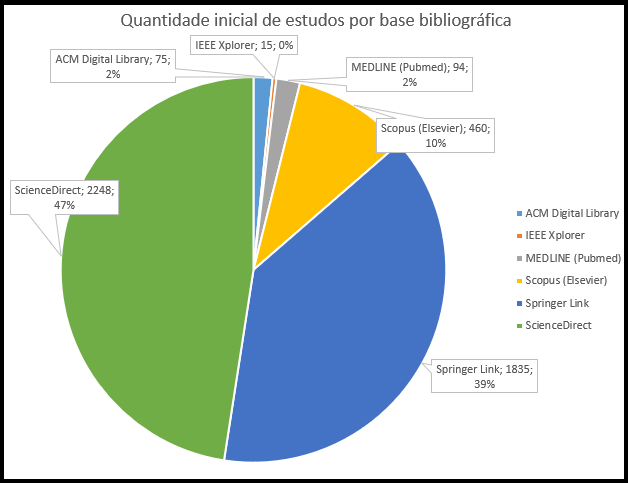
\includegraphics[scale=0.55]{Imagens/grafico - selecao inicial de estudos por base.png}
	\end{center}
	\legend{Fonte: Autor.}
\end{figure}

Porém o termo \textit{nutrition} resultou em uma grande quantidade de estudos relacionados à técnicas de nutrição animal e medições de nutrientes vegetais, que não são relevantes para este trabalho. Estes resultados foram avaliados por seus resumos na etapa de inclusão e 2.625 estudos não foram incluídos para avaliações mais significativas. É possível conferir o comparativo de resultados por strings de busca na \autoref{fig_graficoSelecaoInicialEstudosStrings}.

\begin{figure}[htb]
	\caption{\label{fig_graficoSelecaoInicialEstudosStrings}Gráfico de seleção inicial de estudos por \textit{strings} de busca.}
	\begin{center}
	    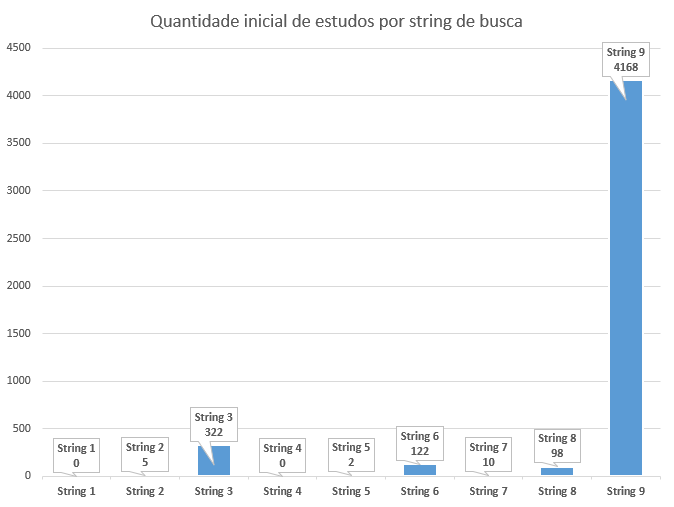
\includegraphics[scale=0.63]{Imagens/grafico - selecao inicial de estudos por string.png}
	\end{center}
	\legend{Fonte: Autor.}
\end{figure}

\begin{figure}[htb]
	\caption{\label{fig_graficoProcessoInclusaoExclusaoArtigos}Gráfico do processo de seleção dos estudos.}
	\begin{center}
	    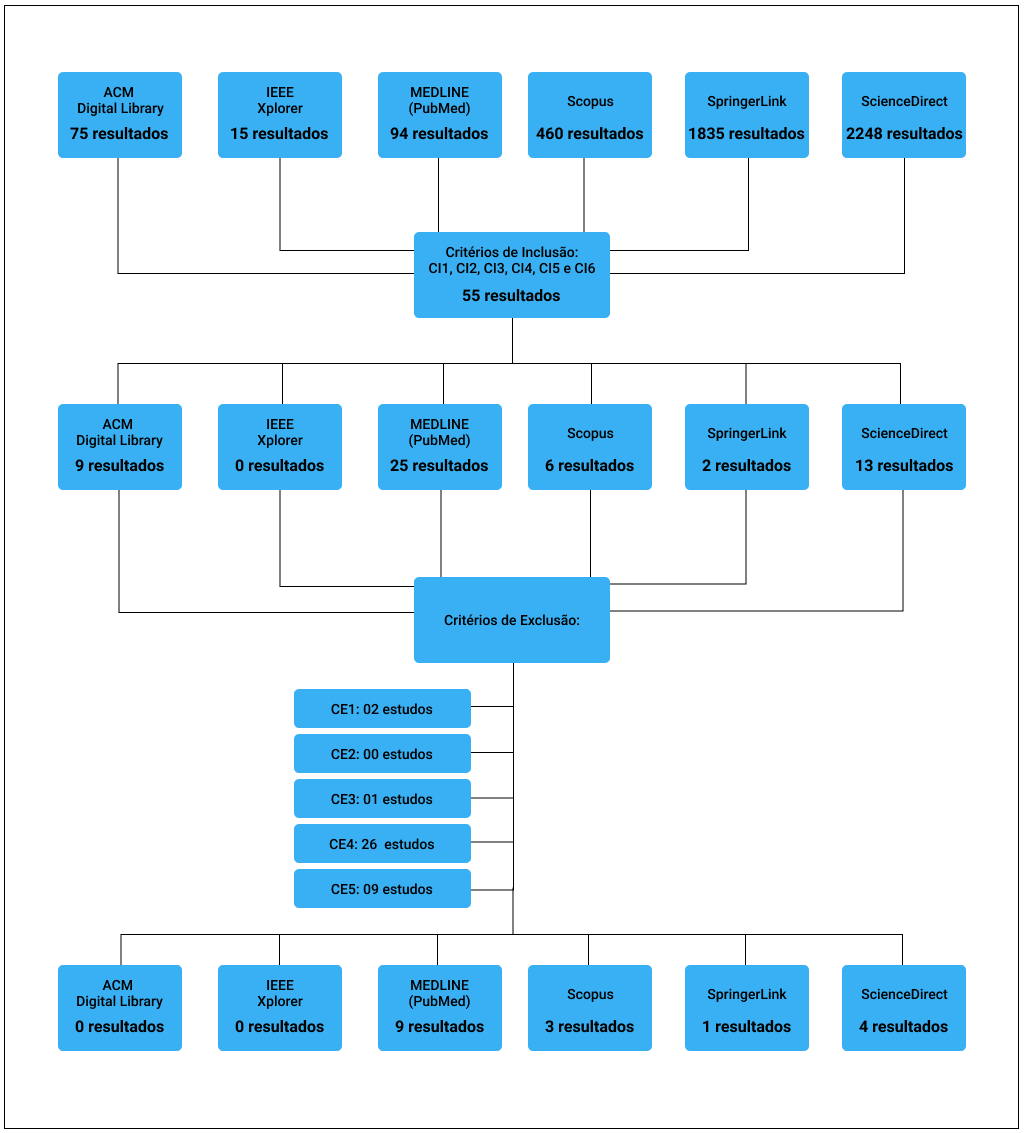
\includegraphics[scale=0.45]{Imagens/grafico - processo de selecao dos estudos.png}
	\end{center}
	\legend{Fonte: Autor.}
\end{figure}

\begin{figure}[htb]
	\caption{\label{fig_graficoResultadoProcessoExclusao}Resultado do processo de exclusão dos artigos.}
	\begin{center}
	    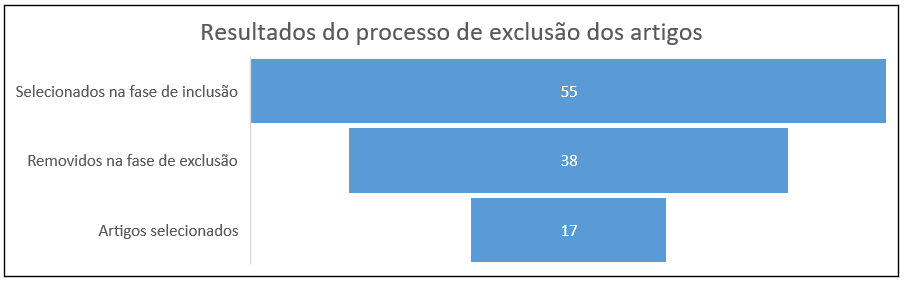
\includegraphics[scale=0.6]{Imagens/grafico - resultado da fase de exclusao dos artigos.png}
	\end{center}
	\legend{Fonte: Autor.}
\end{figure}

Após a execução da busca inicial de estudos, na etapa seguinte analisando os títulos e resumos, 54 resultados satisfizeram ao menos um dos critérios de inclusão e foram selecionados como estudos primários, como mostra a \autoref{fig_graficoProcessoInclusaoExclusaoArtigos}. 
\newline
\newline

Na etapa de exclusão, mostrada na \autoref{fig_graficoProcessoInclusaoExclusaoArtigos}, os artigos que foram coincidentes com ao menos um dos critérios de exclusão foram removidos da revisão. Do total de estudos primários, 26 resultados foram retirados por estarem duplicados, 11 estudos foram removidos por não tratarem do tema abordado neste trabalho e 17 artigos foram selecionados. A \autoref{fig_graficoResultadoProcessoExclusao} apresenta a quantidade total de artigos excluídos e aceitos para análise e extração dos dados. Os artigos selecionados são apresentados no \autoref{quadro_artigosSelecionados}, a seguir.

\begin{quadro}[htb]
\caption{\label{quadro_artigosSelecionados}Artigos selecionados.}
\label{}
\begin{tabular}{|p{1,5cm}|p{7cm}|p{5cm}|}
	\hline
	\textbf{Sigla} & \textbf{Título} & \textbf{Autores} \\ \hline
	A1  & \textit{A dietary assessment app for hospitalized patients at nutritional risk:Development and evaluation of the myfood app} & \cite{paulsen2018_1} \\ \hline
	A2  & \textit{A Parenteral Protein Decision Support System Improves Protein Delivery in Preterm Infants: A Randomized Clinical Trial} & \cite{alrifai2017} \\ \hline
	A3  & \textit{A validation of an intelligent decision-making support system for the nutrition diagnosis of bariatric surgery patients} & \cite{cruz2017} \\ \hline
	A4  & \textit{Advancing competitive position in healthcare: a hybrid metaheuristic nutrition decision support system} & \cite{ileri2019} \\ \hline
	A5  & \textit{Assessing the feasibility of a mobile health-supported clinical decision support system for nutritional triage in oncology outpatients using Arden Syntax} & \cite{bruin2018} \\ \hline
	A6  & \textit{Barriers and Facilitators for Implementing a Decision Support System to Prevent and Treat Disease-Related Malnutrition in a Hospital Setting: Qualitative Study} & \cite{paulsen2018_2} \\ \hline
	A7  & \textit{Clinical Data Warehousing for Evidence Based Decision Making} & \cite{narra2015} \\ \hline
\end{tabular}
\end{quadro} 

\begin{quadro}[htb]
%\caption{(Continuação)}
%\label{}
\begin{tabular}{|p{1,5cm}|p{7cm}|p{5cm}|}
    \hline
	A8  & \textit{Concurrence of big data analytics and healthcare: A systematic review}& \cite{metha2018} \\ \hline
	A9  & \textit{Developing a standardized healthcare cost data warehouse} & \cite{visscher2017} \\ \hline
	A10  & \textit{E-assisted Nutrition Package for Hypertension Patients}& \cite{boonapai2016} \\ \hline
	A11 & \textit{Effects of using the MyFood decision support system on hospitalized patients' nutritional status and treatment: A randomized controlled trial} & \cite{paulsen2020} \\ \hline
	A12  & \textit{Impact of a computer-assisted decision support system (CDSS) on nutrition management in critically ill hematology patients: the NUTCHOCO study (nutritional care in hematology oncologic patients and critical outcome)} & \cite{ettori2019} \\ \hline
	A13  & \textit{Nutritional Alert in hospitalized patients} & \cite{brieux2014} \\ \hline
	A14  & \textit{Physicians' perceptions about managing enteral nutrition and the implementation of tools to assist in nutritional decision-making in a paediatric intensive care unit}& \cite{moullet2020} \\ \hline
	A15  & \textit{Requirements Analysis for a Clinical Decision Support System Aiming at Improving the Artificial Nutrition of Critically Ill Patients}& \cite{schuttler2017} \\ \hline
	A16  & \textit{Using a Web-Based Nutrition Algorithm in Hemodialysis Patients} & \cite{steiber2015} \\ \hline
	A17  & \textit{Using clinical decision support through the electronic medical record to increase prescribing of high-dose parenteral thiamine in hospitalized patients with alcohol use disorder} & \cite{wai2019} \\ \hline
\end{tabular}
\fonte{Autor.}
\end{quadro} 

Os artigos analisados pertencem a uma faixa de publicação entre os anos de 2014 e 2020. Na \autoref{fig_graficoQuantidadeArtigoAno} é apresentado um gráfico com a quantidade de artigos analisados por ano de publicação.
\newline
\newline
\newline
\newline
\newline
\newline
\newline

\begin{figure}[htb]
	\caption{\label{fig_graficoQuantidadeArtigoAno}Quantidade de artigos por ano de publicação.}
	\begin{center}
	    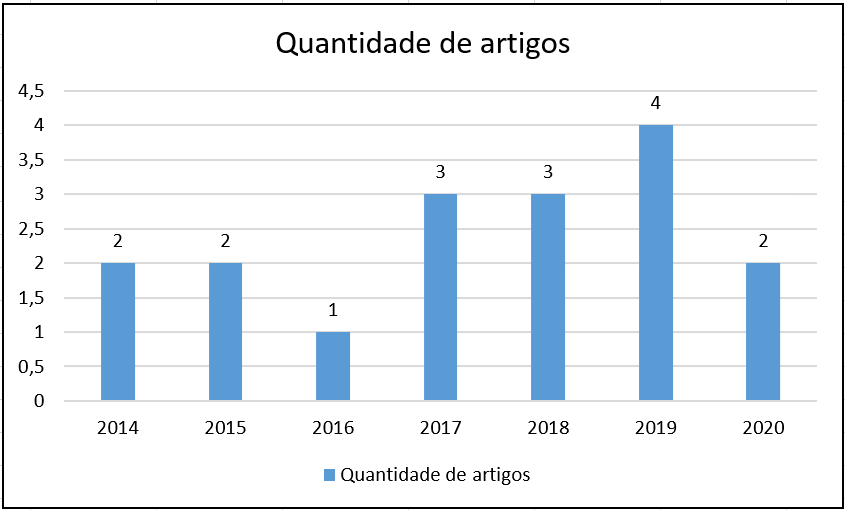
\includegraphics[scale=0.6]{Imagens/grafico - quantidade de artigos por ano de publicacao.png}
	\end{center}
	\legend{Fonte: Autor.}
\end{figure}

A maior quantidade de artigos analisados foram publicados no ano de 2019, com um total de 4 (quatro) artigos. Os anos de 2017 e 2018 apresentaram a segunda maior quantidade de publicações, sendo 3 (três) artigos em cada ano. Seguidos dos anos de 2014, 2015 e 2020 com 2 (dois) artigos em cada ano. E 1 (um) artigo no ano de 2016.

\section{Análise dos resultados}
Na fase de análise, uma vez selecionados os estudos, foi realizada a extração de informações relevantes. Esta seção apresenta as respostas obtidas para as questões de pesquisa. O \autoref{quadro_funcionalidadesArtigos} mostra as principais abordagens encontradas e as formas utilizadas para gerenciamento dos dados.

\textit{µ1: Como as pesquisas tratam o gerenciamento e a análise dos dados clínicos sobre o acompanhamento nutricional dos pacientes nos hospitais?}

\begin{quadro}[htb]
\caption{\label{quadro_funcionalidadesArtigos}Identificação das abordagens de gerenciamento e análise.}
\label{}
\begin{tabular}{|p{11cm}|p{4cm}|}
	\hline
	\textbf{Abordagem utilizada}   &   \textbf{Artigos}\\ \hline
	Apresenta relatório de dados probabilísticos gerados com redes Bayesianas.   &   A3, A4.\\ \hline
	Utiliza algoritmo genético e algoritmo de cozimento simulado para gerar recomendações nos relatórios.  &   A4.\\ \hline
	Utiliza dispositivo móvel apresentar dados de avaliação nutricional. & A1, A5, A6, A11.\\ \hline
	Apresenta \textit{Dashboard} com dados das avaliações nutricionais. & A1, A5, A10, A15, A17.\\ \hline
\end{tabular}
\end{quadro}

\begin{quadro}[htb]
\begin{tabular}{|p{11cm}|p{4cm}|}
    \hline
    Utiliza aplicação web para apresentar dados de avaliação nutricional. & A1, A5, A6, A10, A11.\\ \hline
	Possui estrutura de armazenamento de dados em\textit{ Data Warehouse}. & A7, A11.\\ \hline
	Utiliza \textit{plugin} para apresentar dados de avaliação nutricional.  & A2.\\ \hline
\end{tabular}
\fonte{Autor.}
\end{quadro}

Buscando responder a segunda questão de pesquisa, o \autoref{quadro_indicadoresArtigos} apresenta os formatos de aquisição dos \textit{key performance indicators} utilizados pelos estudos.

\textit{µ2: Como os hospitais extraem indicadores-chave de desempenho (ICP) para análise de dados de acompanhamento nutricional?}

\begin{quadro}[htb]
\caption{\label{quadro_indicadoresArtigos}Formatos de aquisição de Indicadores-chave de desempenho.}
\label{}
\begin{tabular}{|p{11cm}|p{4cm}|}
	\hline
	\textbf{Abordagem utilizada}   &   \textbf{Artigos}\\ \hline
	Utiliza formulário integrado ao módulo de apoio a decisão. &  A2\\ \hline
	Utiliza dispositivo móvel para realizar preenchimento dos dados de avaliação nutricional. & A6, A11\\ \hline
	Utiliza aplicação web para realizar preenchimento de formulário dos dados de avaliação nutricional. & A1, A5 A10, A11\\ \hline
	Utiliza planilha eletrônica para carga de dados & A4, A7.\\ \hline
	Utiliza consulta a base de dados do sistema de administração hospitalar. & A10, A11, A12 A16, A17.\\ \hline
\end{tabular}
\fonte{Autor.}
\end{quadro}

O \autoref{quadro_ImpactosPositivos} apresenta a síntese sobre os impactos que cada artigo causou em seus respectivos ambientes de estudo. 
\newline

\textit{µ3: De que forma esses dados são utilizados e impactam na tomada de decisão dos setores assistenciais e de gestão dos estabelecimentos hospitalares?}

\begin{quadro}[htb]
\caption{\label{quadro_ImpactosPositivos}Síntese sobre os impactos positivos e negativos extraídos nos estudos.}
\label{}
\begin{tabular}{|p{1,5cm}|p{13,5cm}|}
	\hline
	\textbf{Artigo}   &   \textbf{Impactos}\\ \hline
	A1  &  Segundo \citeonline{paulsen2018_1} os dados fornecidos podem contribuir para prevenir o desenvolvimento de desnutrição relacionada à doença entre pacientes em risco.\\ \hline
	A2  &  Para \citeonline{alrifai2017} os principais pontos positivos foram o aumento significativo na dosagem apropriada, a melhora de uremia e o ganho de peso durante fase de nutrição enteral.\\ \hline
	A3  &  \citeonline{cruz2017} apresentam grande vantagem na sugestão baseada de risco de desenvolvimento de doença baseado no relatório.\\ \hline
	A4  & \citeonline{ileri2019} analisam os pedidos do menu de dieta e sugere vários menus para fornecer eficácia de custo e possíveis taxas de erro mais baixas ao mesmo tempo.\\ \hline
\end{tabular}
\end{quadro}
\newpage
\begin{quadro}[htb]
\begin{tabular}{|p{1,5cm}|p{13,5cm}|}
    \hline
	A5  &  \citeonline{bruin2018} apresentam um monitoramento que pode servir como o elo que faltava na identificação precoce de mudança no estado nutricional de um paciente.\\ \hline
    A6  & \citeonline{paulsen2018_2} apresentam um aplicativo móvel para acompanhamento nutricional de pacientes hospitalizados, que foi percebido pelo usuários como mais preciso, confiável, divertido e motivacional do que a prática tradicional. Contudo,
    aspectos culturais, de idioma, idade, higiene e falta de integração com sistema de prontuários foram percebidos como barreiras potenciais. \\ \hline
    A7 & \citeonline{narra2015} consideram a vantagem de integrar diferentes fontes de dados para possibilitar análise dimensional. Além disso, a natureza não volátil dos \textit{data warehouses} permitem o estudo de vários fatores e problemas de saúde que só podem ser identificados com dados de um longo período de tempo além da possibilidade de aplicar técnicas de mineração de dados.\\ \hline
    A8 & \citeonline{metha2018} apresentam como o sistema de apoio a decisão ajuda na detecção precoce de doenças, dicção da trajetória da doença e identificação de desvio de estado saudável. O tratamento direcionado pode ser direcionado ajudando as organizações de saúde em custo-benefício e redução do desperdício de recursos.\\ \hline
    A9 & Em \citeonline{visscher2017}, um \textit{data warehouse} padronizado e baseado em provedor de dados de custos de saúde pode ser mantido facilmente. Sendo útil para fornecer estimativas de custo total razoáveis e compreensíveis, entendo melhor o faturamento e possibilitando estratégias que melhorem o custo-beneficio por paciente na rede hospitalar.\\ \hline
    A10 & \citeonline{boonapai2016} implementam com sucesso um modelo de consciência nutricional e orientação para o usuário, especialmente com hipertensão, diabetes e obesidade, porque podem controlar e monitorar sua condição e seus planos de dieta.\\ \hline
    A11 & \citeonline{paulsen2020} obtiveram um efeito significativo na proporção de pacientes com tratamento nutricional documentado no prontuário eletrônico do paciente.\\ \\ \hline
    A12 & \citeonline{ettori2019} mostraram melhorar relativamente a taxa de dias no cumprimento das metas calóricas e proteicas em mais de 50\%.\\ \hline
    A13 & O sistema de alerta apresentado por \citeonline{brieux2014} teve alta sensibilidade e especificidade e esse fato ajudou os médicos a diagnosticarem a desnutrição nos pacientes.\\ \hline
    A14 & Médicos relataram práticas mais consistentes e sistemáticas, segundo \citeonline{moullet2020}, como por exemplo, a determinação de metas de energia na admissão na Unidade de Terapia Intensiva Pediátrica e maior atenção à nutrição.\\ \hline
    A15 &  \citeonline{schuttler2017} propuseram três camadas de visualização, o que permitiu ao usuário obter as informações necessárias e, simultaneamente, evitar a sobrecarga de informações.\\ \hline
    A16 & \citeonline{steiber2015} apresentaram a capacidade de rastrear mudanças nas medidas de avaliação ao longo do tempo. \\ \hline
\end{tabular}
\end{quadro}
\newpage
\begin{quadro}[htb]
\begin{tabular}{|p{1,5cm}|p{13,5cm}|}
    A17 & O trabalho realizado por \citeonline{wai2019} resultou em um aumento significativo na prescrição de tiamina parenteral em alta dose e uma tendência à significância estatística para diminuir o tempo de internação. \\ \hline
\end{tabular}
\fonte{Autor.}
\end{quadro}
Também buscando responder a terceira questão de pesquisa, foi identificada a densidade de KPI's utilizadas nos artigos, conforme a \autoref{fig_graficoDensidadeKPI}.

\begin{figure}[htb]
	\caption{\label{fig_graficoDensidadeKPI}Quantidade de artigos por ano de publicação.}
	\begin{center}
	    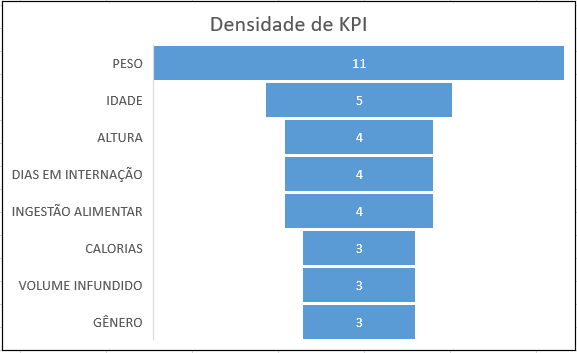
\includegraphics[scale=0.8]{Imagens/grafico - densidade de kpi.png}
	\end{center}
	\legend{Fonte: Autor.}
\end{figure}


\section{Considerações do capítulo}
Este capítulo descreveu a execução de cada etapa do processo da revisão sistemática. Esta revisão teve como objetivo conhecer as pesquisas que trataram do apoio a tomada de decisão na área da nutrição hospitalar. Foi apresentado o processo de planejamento e realização da execução da revisão, por fim, realizada a extração dos dados, obtendo principais abordagens de gerenciamento e analise dos dados, formas de extração e principais \textit{KPI's} utilizados em projetos de sistemas de apoio a decisão. No próximo capítulo será descrito o desenvolvimento do Sistema de Apoio a Decisão da Unidade de Nutrição do HU.
% ---
% Capitulo de Desenvolvimento da Aplicação
% ---
\chapter{Desenvolvimento}
% ---
Este capítulo apresenta o projeto do \textit{Business Intelligence} do Setor de Nutrição Clínica do HU-UFS abordando estratégias, necessidades informacionais e peculiaridades do setor de nutrição do hospital. Serão descritas as atividades de criação do modelo relacional do \textit{Datawarehouse}, detalhamento do processo de ETL e a elaboração da interface OLAP. São apresentados também a interface web destinada aos tomadores de decisão, os resultados das consultas OLAP e informações referentes ao escopo do projeto e ao HU-UFS.
% ---
\section{Hospital Universitário de Aracaju - HU-UFS}
% ---
O Hospital Universitário (HU) é um campus da Universidade Federal de Sergipe (UFS) desde 1984, funcionando como centro hospitalar de assistência, ensino e pesquisa em ciências da saúde. Atualmente, o HU-UFS em Sergipe ocupa um espaço de referência e excelência na prestação de assistência médico-hospitalar de média e alta complexidade \cite{sitehuufs}.

Em 2013, a UFS e a Empresa Brasileira de Serviços Hospitalares (EBSERH) firmaram convênio para transferência da administração do HU no âmbito do Programa Nacional de Reestruturação dos Hospitais Universitários Federais (REHUF). O HU-UFS tornou-se a nona filial da EBSERH com administração vigorosa em todas as áreas do hospital. Em abril de 2016, o HU-UFS tornou-se habilitado para o atendimento especializado de pessoas com deficiência auditiva, bem como para procedimentos de vasectomia. Atualmente, a estrutura do hospital inclui departamentos de Clínica Médica, Clínica Cirúrgica, Pediatria, Unidade de Terapia Intensiva (UTI) e Centro Cirúrgico. Vários cursos de graduação, pós-graduação, residência médica e multiprofissional utilizam as instalações desse hospital-escola para desenvolver práticas e pesquisas inovadoras \cite{sitehuufs}. 

% ---
\section{Escopo do Projeto}
% ---
A Unidade de Nutrição Clínica do HU armazena seus registros de formulários de acompanhamento nutricional dos pacientes em planilhas eletrônicas. As informações entregues à gestão do hospital são consultadas nestas planilhas pela chefia do setor. Os dados mais relevantes para a chefia estão relacionadas aos índices de classificação de risco, estado nutricional, utilização de suplementação e utilização de dietas enterais e suas relações com possíveis complicações identificadas nos pacientes internados nas diversas clínicas do hospital. Um dos formulários utilizados para coleta de dados básicos para essas planilhas é apresentado na \autoref{fig_figuraFormularioDiagClinicoNutri}.

\begin{figure}[htb]
	\caption{\label{fig_figuraFormularioDiagClinicoNutri}Formulário de Diagnóstico Clínico-Nutricional.}
	\begin{center}
	    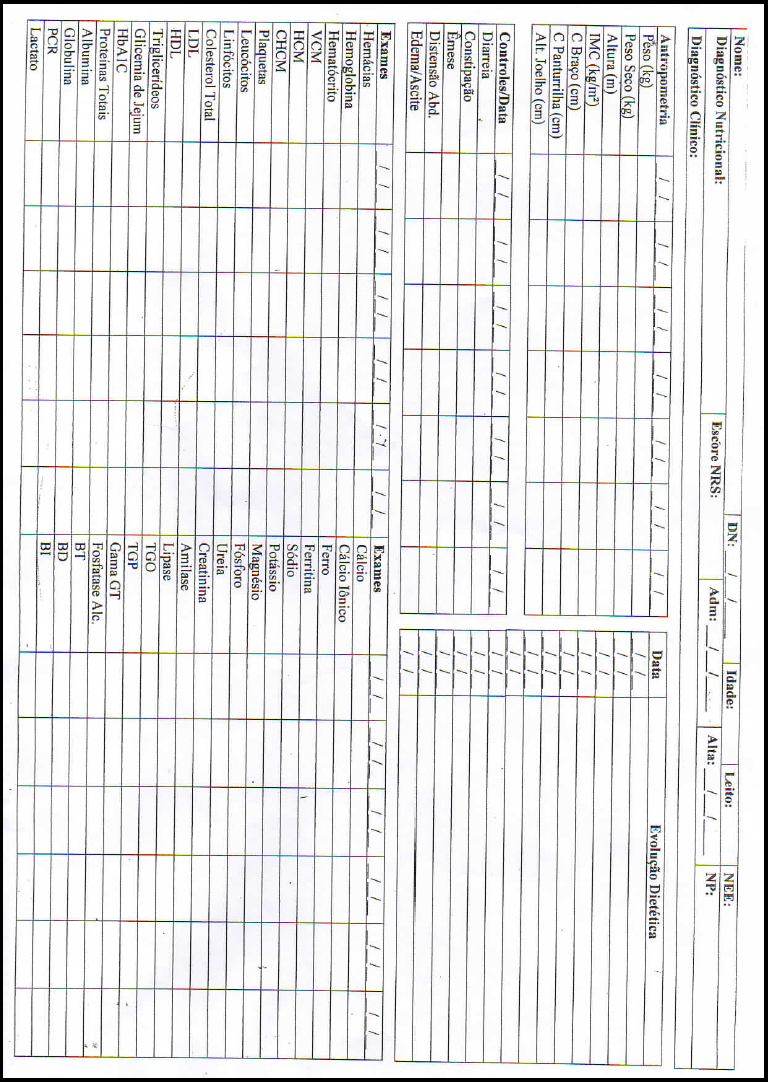
\includegraphics[scale=0.569]{Imagens/figura - formulario diagnostico clinico nutricional.png}
	\end{center}
	\legend{Fonte: \cite{huufs}.}
\end{figure}

Todos esses dados, antes de serem carregados no \textit{Data Warehouse} (DW) devem passar por um processo de ETL, que de forma sistemática realiza tratamento e limpeza dos dados advindos dos diversos arquivos fornecidos pela unidade de nutrição e pelo hospital. 

Um ponto importante a ser considerado, é que devido ao surto mundial de Sars-Cov-2, confirmado pela \citeonline{whocovid} em 2020, vários hospitais tiveram de passar por revisões dos seus protocolos de atendimento. Com a emissão de resolução do Conselho Federal de Nutrição e do Protocolo Operacional Padrão emitido pelo HU-UFS, a Unidade de Nutrição não mais realizou triagens nutricionais em pacientes de forma presencial e o acompanhamento nutricional foi realizado apenas de forma online e com regras diferentes para avaliação \cite{protocolocovidnutri, cfnutri646}. Com todas as mudanças ocorridas em 2020, a unidade não foi capaz de realizar o registro de alguns dados conforme padrão de anos anteriores e disponibilizou apenas a fonte de dados do ano de 2019 para consideração neste trabalho.

Com os dados disponíveis carregados no DW se faz necessário criar um modelo de dados OLAP, no qual as informações são organizadas conceitualmente em cubos de dados para análise dinâmica e multidimensional dos dados consolidados.

Com a possibilidade de consultas dinâmicas oferecidas pelo OLAP a Unidade de Nutrição Clínica solicitou além dos dados quantitativos também gráficos de comparação, composição e tendência para diferentes dimensões, sempre considerando uma visão de todo o hospital e uma visão por enfermaria como descritos abaixo: 

Para o indicador de Triagem Nutricional Realizada, as seguintes informações foram solicitados:
\begin{itemize}
    \item Quantidade de Triagens Nutricionais Realizadas ao Ano;
    \item Quantidade de Triagens Nutricionais Realizadas por Mês;
    \item Quantidade de Triagens Nutricionais Realizadas por Enfermaria ao Ano;
    \item Tendência de Triagens Nutricionais Realizadas por Enfermaria.
\end{itemize}

Para o indicador de Classificação de Risco foram solicitadas as seguintes informações:
\begin{itemize}
    \item Percentual de Pacientes segundo Classificação de Risco ao Ano;
    \item Percentual de Pacientes segundo Classificação de Risco detalhado por mês;
    \item Percentual de Pacientes segundo Classificação de Risco por Enfermaria ao Ano;
    \item Tendência de Pacientes segundo Classificação de Risco por Enfermaria detalhado por mês.
\end{itemize}

Para o indicador de Estado Nutricional foram solicitadas as seguintes informações:
\begin{itemize}
    \item Percentual de Pacientes segundo Estado Nutricional ao Ano;
    \item Percentual de Pacientes segundo Estado Nutricional detalhado por mês;
    \item Percentual de Pacientes segundo Estado Nutricional por Enfermaria ao Ano;
    \item Tendência de Pacientes segundo Estado Nutricional por Enfermaria detalhado por mês.
\end{itemize}

Para o indicador de Uso de Suplementação foram solicitadas as seguintes informações:
\begin{itemize}
    \item Quantidade de Pacientes em Uso de Suplemento;
    \item Quantidade de Pacientes em Uso de Suplemento por Enfermaria;
    \item Percentual de Pacientes segundo Uso de Suplementação ao Ano;
    \item Percentual de Pacientes segundo Uso de Suplementação por Enfermaria ao Ano;
    \item Tendência de Pacientes segundo Uso de Suplementação por Enfermaria detalhado por mês;
    \item Comparativo de pacientes que utilizam Suplementação com média de dias internado;
    \item Comparativo de pacientes que utilizam Suplementação com média de dias internado por enfermaria.
\end{itemize}

Para o indicador de Insumo foi solicitada a seguinte informação:
\begin{itemize}
    \item Percentual de Insumos utilizados por Enfermaria;
\end{itemize}

Para o indicador de Uso de Dieta Enteral foram solicitadas as seguintes informações:
\begin{itemize}
    \item Quantidade de Pacientes em Uso de Dieta Enteral;
    \item Quantidade de Pacientes em Uso de Dieta Enteral por Enfermaria;
    \item Percentual de Pacientes segundo Uso de Dieta Enteral ao Ano;
    \item Percentual de Pacientes segundo Uso de Dieta Enteral por Enfermaria ao Ano;
    \item Tendência de Pacientes segundo Uso de Dieta Enteral por Enfermaria detalhado por mês;
    \item Comparativo de pacientes que utilizam Dieta Enteral com média de dias internado;
    \item Comparativo de pacientes que utilizam Dieta Enteral com média de dias internado por enfermaria.
\end{itemize}

Para o indicador de Complicações, que podem ocorrer por Uso de Suplementação e Uso de Dieta Enteral foram solicitadas as seguintes informações:
\begin{itemize}
    \item Percentual de Complicações em Uso de Suplementação ao Ano;
    \item Percentual de Complicações em Uso de Suplementação por Enfermaria ao Ano;
    \item Percentual de Complicações em Uso de Dieta Enteral ao Ano;
    \item Percentual de Complicações em Uso de Dieta Enteral por Enfermaria ao Ano;
\end{itemize}

Para o indicador de Desfecho onde podem ocorrer altas, transferências ou óbitos, combinado a Dimensão de Classificações de Risco foram solicitadas as seguintes informações:
\begin{itemize}
    \item Percentual de Desfecho por Classificação de Risco ao Ano;
    \item Percentual de Desfecho por Classificação de Risco por Enfermaria ao Ano;
\end{itemize}

\section{Ambiente de \textit{Business Intelligence}}

O ambiente BI escolhido utilizou o conjunto de ferramentas \textit{Pentaho Community}, que são mantidas e disponibilizadas gratuitamente pela Hitachi Vantara©. O \textit{Pentaho Community} fornece um pacote de ferramentas completo para soluções BI. Para este trabalho foram utilizadas as seguintes ferramentas: \textit{Pentaho Data Integration, Pentaho Schema Workbench e Pentaho Business Analytics Platform}.

Alguns pré-requisitos são necessários para o bom funcionamento do ambiente. Foram instalados os seguintes softwares auxiliares: Java SE \textit{Runtime Environment} 8 \textit{update} 261, PostgreSQL 12.5, PG Admin 4.24 e SQL \textit{Power Arquitect} 1.0.8. Ainda nesta seção são descritas as etapas de modelagem multidimensional do \textit{Data Warehouse} e do \textit{Data Mart}, o processo de ETL, o mapeamento lógico do cubo de dados OLAP, as consultas e os resultados dos \textit{Dashboards}.

\subsection{Modelagem Multidimensional}
Ao analisar as características das informações solicitadas pela gestão da unidade de nutrição, considerando cada necessidade como um problema a ser resolvido, foi concebido do modelo multidimensional usando a estrutura \textit{star schema}. O esquema foi modelado com 13 dimensões (Hospital, Enfermaria, Tempo, Paciente, Classificação Nutricional, Estado Nutricional, Complicações, Triagem Realizada, Suplementação, Dieta Enteral, Insumos, Edema e Desfecho) e uma Fato (Nutrição). A \autoref{fig_modelagemdatawarehouse} mostra o modelo de dados do \textit{Data Warehouse} projetado neste trabalho.

\begin{figure}[htb]
	\caption{\label{fig_modelagemdatawarehouse}Modelo Multidimensional do Data Warehouse.}
	\begin{center}
	    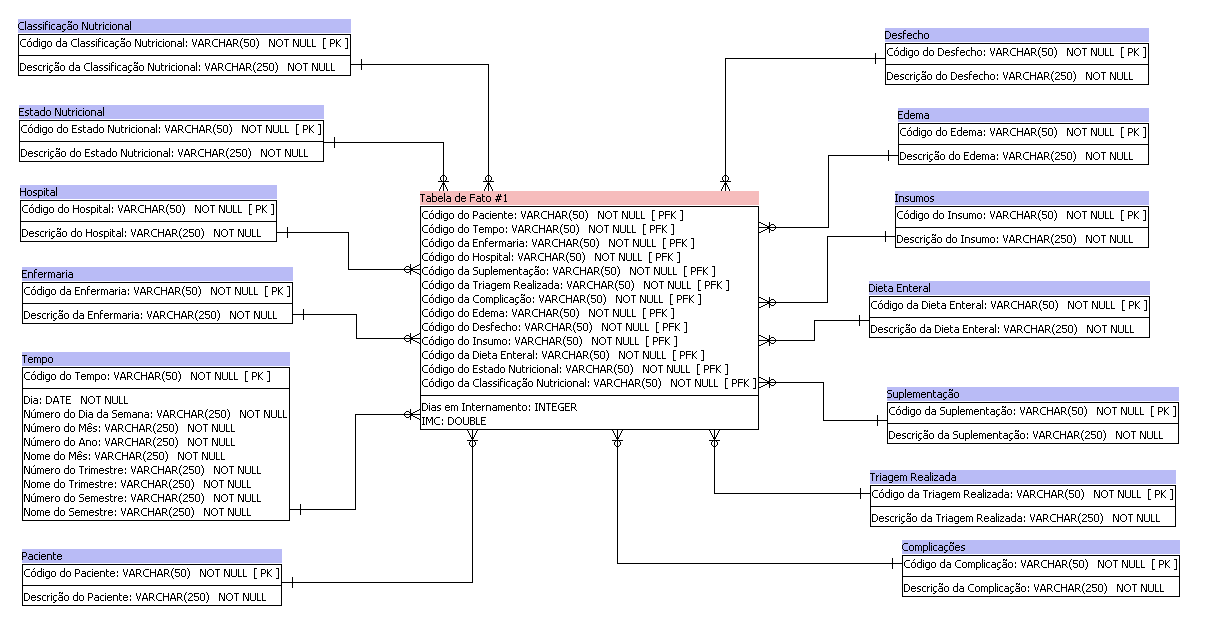
\includegraphics[scale=0.5]{Imagens/figura - modelagem multidimensional datawarehouse.png}
	\end{center}
	\legend{Fonte: Autor.}
\end{figure}

Com o objetivo de permitir melhor performance para as consultas também foi projetado um cubo OLAP de modelo relacional, mais especificamente chamado de \textit{Relational Online Analitycal Processing} (ROLAP), como é mostrado na \autoref{fig_modelagemdatamart}.

\newpage
\begin{figure}[htb]
	\caption{\label{fig_modelagemdatamart}Modelo Relacional do Data Mart.}
	\begin{center}
	    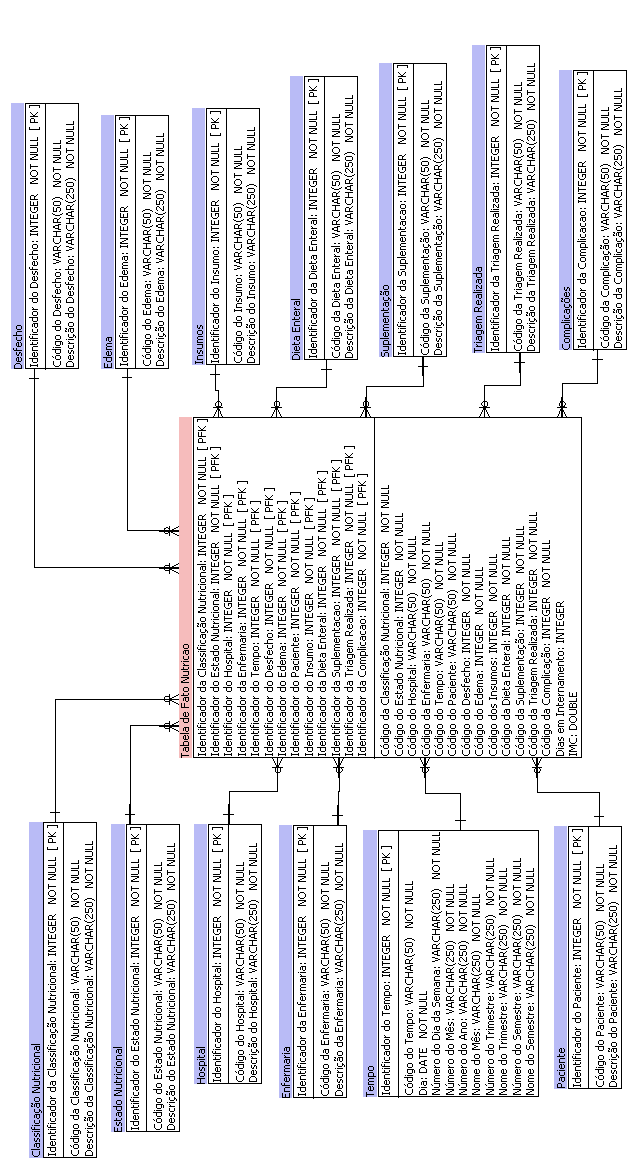
\includegraphics[scale=0.5]{Imagens/figura - modelagem multidimensional datamart.png}
	\end{center}
	\legend{Fonte: Autor.}
\end{figure}

O projeto multidimensional e o projeto do cubo ROLAP foram construídos com a ferramenta SQL \textit{Power Architect}, que além da concepção, auxilia na geração e execução do \textit{script} de criação tanto do \textit{Data Warehouse}, quanto do \textit{Data Mart}, implementados na sintaxe do PostgreSQL. Além de ser um SGBD robusto e gratuito, o PostgreSQL também é o sistema de gerenciamento de banco de dados utilizado pelo HU. 

\subsection{Processo de Extração, Transformação e Carga}
Com o modelo dimensional construído, foi dada sequência à próxima etapa do projeto, o desenvolvimento do processo de extração, transformação e carga. Para a fase de ETL foi utilizado o \textit{Pentaho Data Integration} (PDI), ferramenta da Pentaho utilizada para sistematizar o processo de tratamento e limpeza dos dados oriundos das fontes de dados e inserção nos armazéns de dados e nos \textit{Data Marts}.

A partir dos arquivos disponibilizados pela Unidade de Nutrição, em formato de arquivo de planilha no padrão Open XML adaptado pela Microsoft (XLSX), foram corrigidos, padronizados e tratados todos os desvios e inconsistências encontradas. Sequencialmente é iniciada a carga dos dados no DW, concluindo a persistência dos dados consolidados. Foram desenvolvidos um \textit{script} ETL para cada dimensão e um \textit{script} para a tabela de fato, resultando em 14 \textit{scripts} ETL. A seguir, estão as figuras das transformações utilizadas para a carga completa do DW. 
\newpage

\begin{figure}[htb]
	\caption{\label{fig_etldimensaohospital}Processo ETL para a Dimensão Hospital.}
	\begin{center}
	    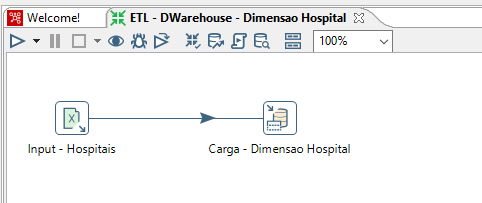
\includegraphics[scale=0.8]{Imagens/figura - etl dw hospital.png}
	\end{center}
	\legend{Fonte: Autor.}
\end{figure}

Na \autoref{fig_etldimensaoenfermaria} os dados relacionados as enfermarias do Hospital Universitário foram consultados do banco de dados do Aplicativo de Gestão para Hospitais Universitários (AGHU). 
\begin{figure}[htb]
	\caption{\label{fig_etldimensaoenfermaria}Processo ETL para a Dimensão Enfermaria.}
	\begin{center}
	    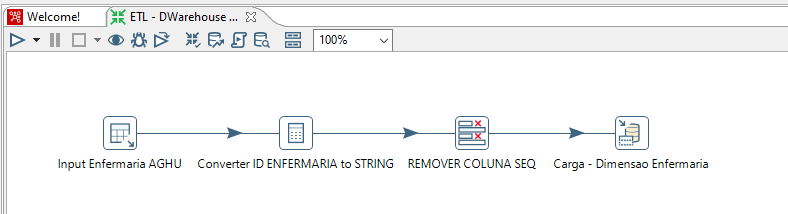
\includegraphics[scale=0.7]{Imagens/figura - etl dw enfermaria.png}
	\end{center}
	\legend{Fonte: Autor.}
\end{figure}

\begin{figure}[htb]
	\caption{\label{fig_etldimensaotriagem}Processo ETL para a Dimensão Triagem Realizada.}
	\begin{center}
	    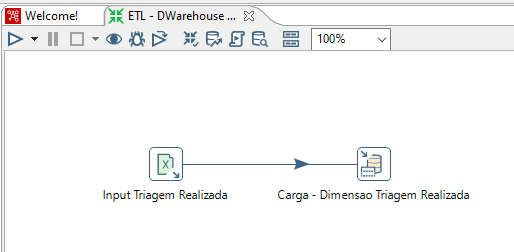
\includegraphics[scale=0.64]{Imagens/figura - etl dw triagem.png}
	\end{center}
	\legend{Fonte: Autor.}
\end{figure}

\begin{figure}[htb]
	\caption{\label{fig_etldimensaotempo}Processo ETL para a Dimensão Tempo.}
	\begin{center}
	    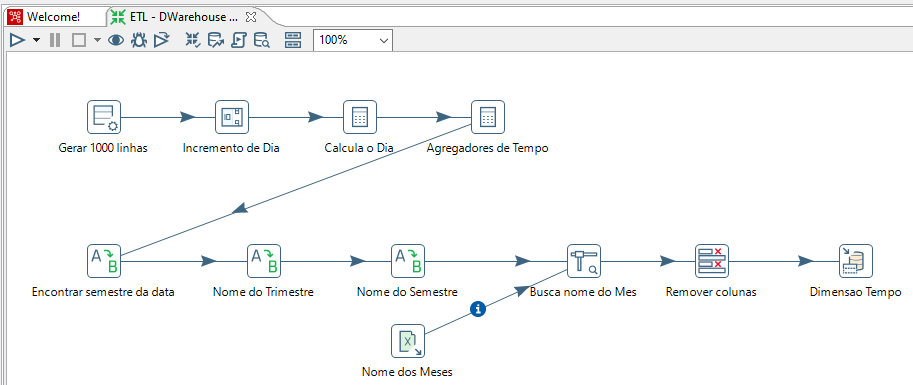
\includegraphics[scale=0.6]{Imagens/figura - etl dw tempo.png}
	\end{center}
	\legend{Fonte: Autor.}
\end{figure}

\begin{figure}[htb]
	\caption{\label{fig_etldimensaopaciente}Processo ETL para a Dimensão Paciente.}
	\begin{center}
	    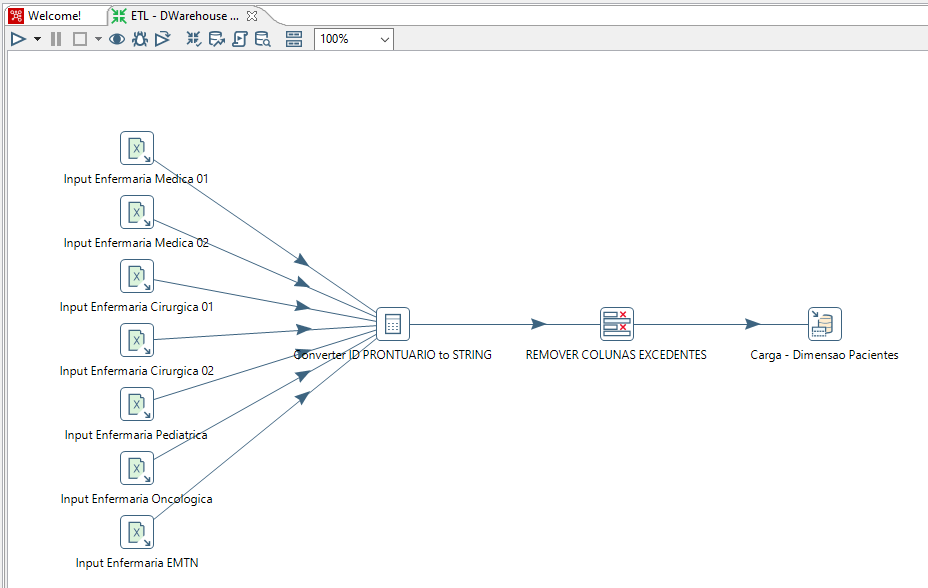
\includegraphics[scale=0.6]{Imagens/figura - etl dw paciente.png}
	\end{center}
	\legend{Fonte: Autor.}
\end{figure}
                    \clearpage
\begin{figure}[htb]
	\caption{\label{fig_etldimensaosuplementacao}Processo ETL para a Dimensão Suplementação.}
	\begin{center}
	    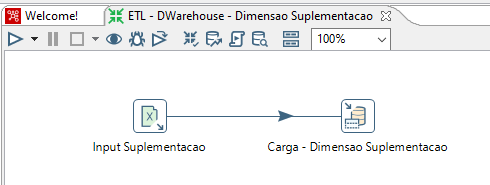
\includegraphics[scale=0.8]{Imagens/figura - etl dw suplementacao.png}
	\end{center}
	\legend{Fonte: Autor.}
\end{figure}

\begin{figure}[htb]
	\caption{\label{fig_etldimensaoinsumo}Processo ETL para a Dimensão Insumos.}
	\begin{center}
	    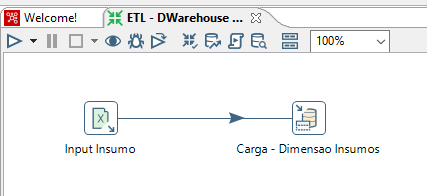
\includegraphics[scale=0.82]{Imagens/figura - etl dw insumos.png}
	\end{center}
	\legend{Fonte: Autor.}
\end{figure}

\begin{figure}[htb]
	\caption{\label{fig_etldimensaoestado}Processo ETL para a Dimensão Estado Nutricional.}
	\begin{center}
	    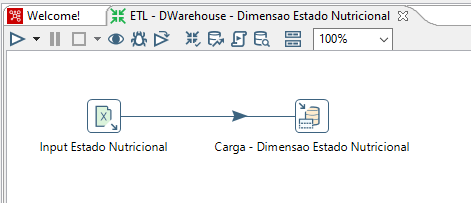
\includegraphics[scale=0.8]{Imagens/figura - etl dw estadonutricional.png}
	\end{center}
	\legend{Fonte: Autor.}
\end{figure}
                    \clearpage
\begin{figure}[htb]
	\caption{\label{fig_etldimensaoedema}Processo ETL para a Dimensão Edema.}
	\begin{center}
	    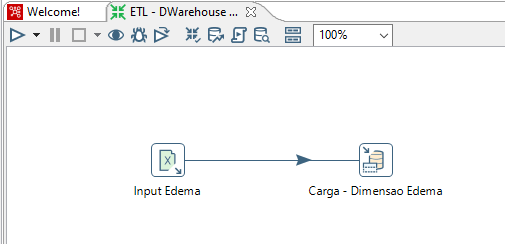
\includegraphics[scale=0.7]{Imagens/figura - etl dw edema.png}
	\end{center}
	\legend{Fonte: Autor.}
\end{figure}

\begin{figure}[htb]
	\caption{\label{fig_etldimensaodesfecho}Processo ETL para a Dimensão Desfecho.}
	\begin{center}
	    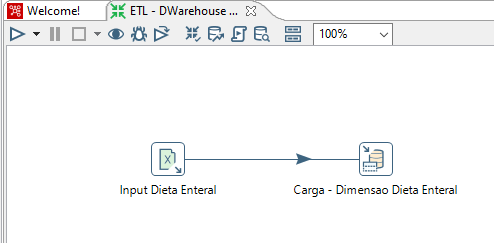
\includegraphics[scale=0.7]{Imagens/figura - etl dw dietaenteral.png}
	\end{center}
	\legend{Fonte: Autor.}
\end{figure}

\begin{figure}[htb]
	\caption{\label{fig_etldimensaocomplicacoes}Processo ETL para a Dimensão Complicações.}
	\begin{center}
	    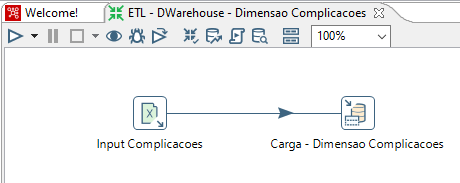
\includegraphics[scale=0.72]{Imagens/figura - etl dw complicacoes.png}
	\end{center}
	\legend{Fonte: Autor.}
\end{figure}
                \clearpage
\begin{figure}[htb]
	\caption{\label{fig_etldimensaoclassificacao}Processo ETL para a Dimensão Classificação Nutricional.}
	\begin{center}
	    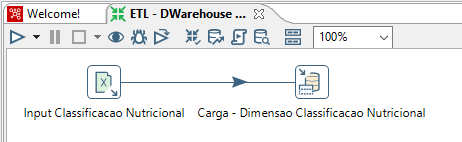
\includegraphics[scale=0.8]{Imagens/figura - etl dw classificacao.png}
	\end{center}
	\legend{Fonte: Autor.}
\end{figure}
A \autoref{fig_etltabelafato} mostra o processo de transformação e carga para a Tabela de Fato do Data Warehouse. 
\begin{figure}[htb]
	\caption{\label{fig_etltabelafato}Processo ETL para a Tabela de Fato do Data Warehouse.}
	\begin{center}
	    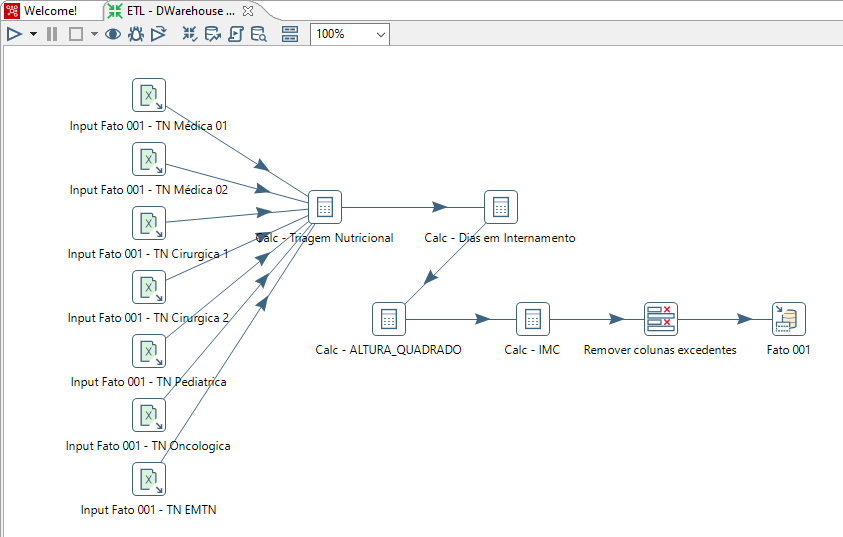
\includegraphics[scale=0.7]{Imagens/figura - etl dw fato.png}
	\end{center}
	\legend{Fonte: Autor.}
\end{figure}

Na \autoref{fig_etlcargafatodatamart} está representado o processo de transformação e carga para a tabela fato do Datamart. Já na \autoref{fig_etlcargadimensoesdatamart} está representado o processo para as dimensões do Datamart.

\begin{figure}[htb]
	\caption{\label{fig_etlcargafatodatamart}Processo ETL para a Tabela de Fato do \textit{Datamart}.}
	\begin{center}
	    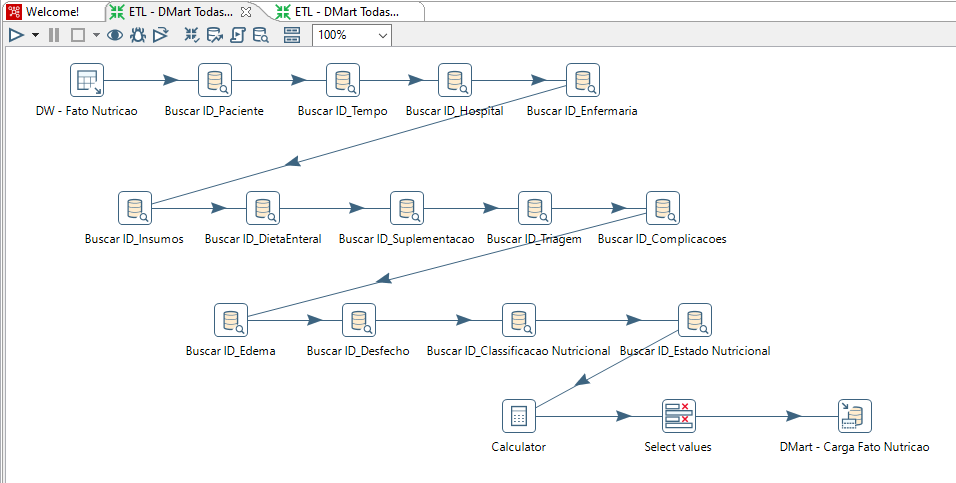
\includegraphics[scale=0.57]{Imagens/figura - etl dm fato.png}
	\end{center}
	\legend{Fonte: Autor.}
\end{figure}

\begin{figure}[htb]
	\caption{\label{fig_etlcargadimensoesdatamart}Processo ETL para as Dimensões do \textit{Datamart}.}
	\begin{center}
	    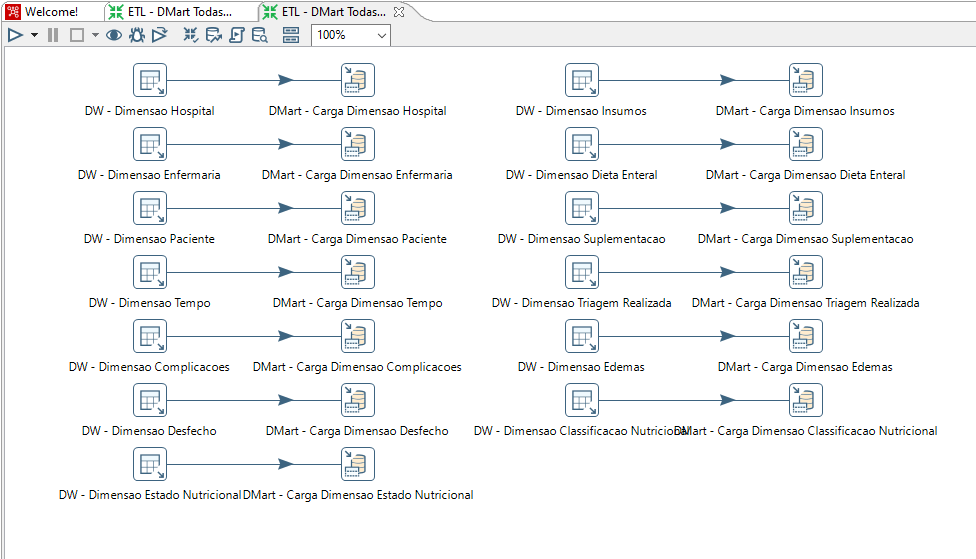
\includegraphics[scale=0.56]{Imagens/figura - etl dm dimensoes.png}
	\end{center}
	\legend{Fonte: Autor.}
\end{figure}
            \clearpage

\subsection{Mapeamento e Consultas OLAP}
Com o processo de carga completo, o próximo passo da sequência é a configuração e criação do cubo lógico de dados com as propriedades das medidas e dimensões, como funções de agregação, formatação, funções matemáticas e nome para exibição. A ferramenta utilizada foi o Pentaho Schema Workbench que também é fornecida no pacote Pentaho Community e usa o mecanismo Modrian para se comunicar com os esquemas ROLAP e processar as solicitações de consultas multidimensionais ou MDX como também são conhecidas na sigla em inglês para \textit{Multidimensional Express}. A \autoref{fig_pentahoshemaworkbench} apresenta o cubo lógico "DMNutricao", onde estão definidas as medidas: "ClassificacaoDeRisco"," EstadoNutricional", "Desfecho", "Edema", "Insumo", "DietaEnteral", "UsoDeSuplemento", "TriagemRealizada", "Complicacoes" e "DiasInternamento" que serão utilizados para geração dos \textit{dashboards}, utilizando todas as Dimensões de acordo com modelo relacional da \autoref{fig_modelagemdatamart}.

\begin{figure}[htb]
	\caption{\label{fig_pentahoshemaworkbench}Modelagem do cubo lógico de dados.}
	\begin{center}
	    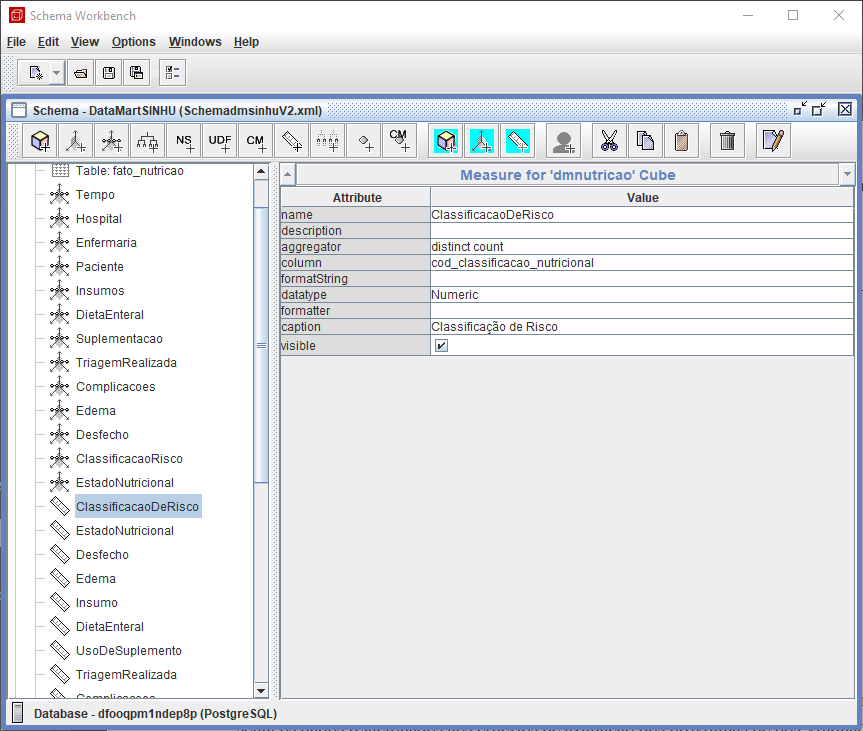
\includegraphics[scale=0.65]{Imagens/figura - schema workbench.png}
	\end{center}
	\legend{Fonte: Autor.}
\end{figure}

As consultas MDX que são a base dos relatórios e gráficos podem ser montadas e testadas no ambiente de query do próprio Schema Workcbench, a \autoref{fig_shemaworkbenchconsulta} mostra a consulta MDX realizada para o relatório de quantidade de triagens realizadas por mês para cada enfermaria do hospital. Na área em amarelo é escrita a query de consulta e na área em vermelho é mostrada a resposta da consulta multidimensional.
\begin{figure}[htb]
	\caption{\label{fig_shemaworkbenchconsulta}Exemplo de consulta MDX no Schema Workbench.}
	\begin{center}
	    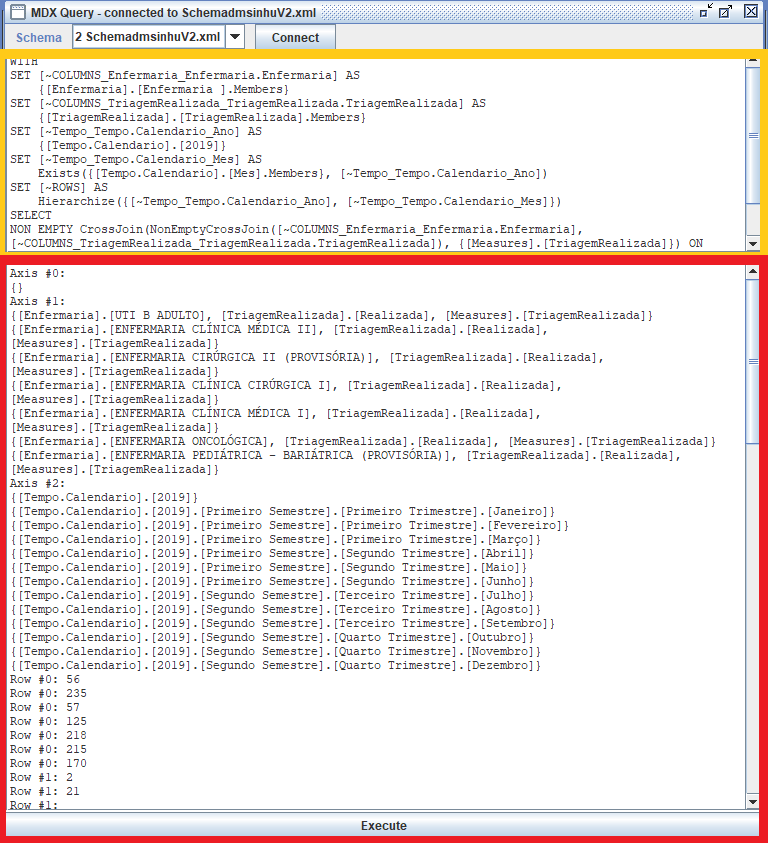
\includegraphics[scale=0.7]{Imagens/figura - workbenchconsulta.png}
	\end{center}
	\legend{Fonte: Autor.}
\end{figure}

\subsection{Ambiente de Relatórios}
Com o ambiente pronto e as consultas necessárias montadas, é possível seguir à etapa de geração dos relatórios e \textit{dashboards} no Pentaho Business Analytics Platform. A plataforma de \textit{Business Analytics} vem com o editor padrão de relatórios JPivot View, mas também é permitida a instalação de outras bibliotecas, que podem ser integradas por meio do \textit{Marketplace} da Pentaho ou instaladas manualmente quando de fontes externas. O JPivot em sua versão disponibilizada de forma padrão no Pentaho Server foi descontinuada e por este motivo para este trabalho foi instalada a biblioteca Saiku Analytics, um cliente web disponível em forma de \textit{plugin} no \textit{Marketplace}, como mostra a \autoref{fig_pluginsaiku}. 
\begin{figure}[htb]
	\caption{\label{fig_pluginsaiku}Plugin Saiku Analytics no Pentaho Marketplace.}
	\begin{center}
	    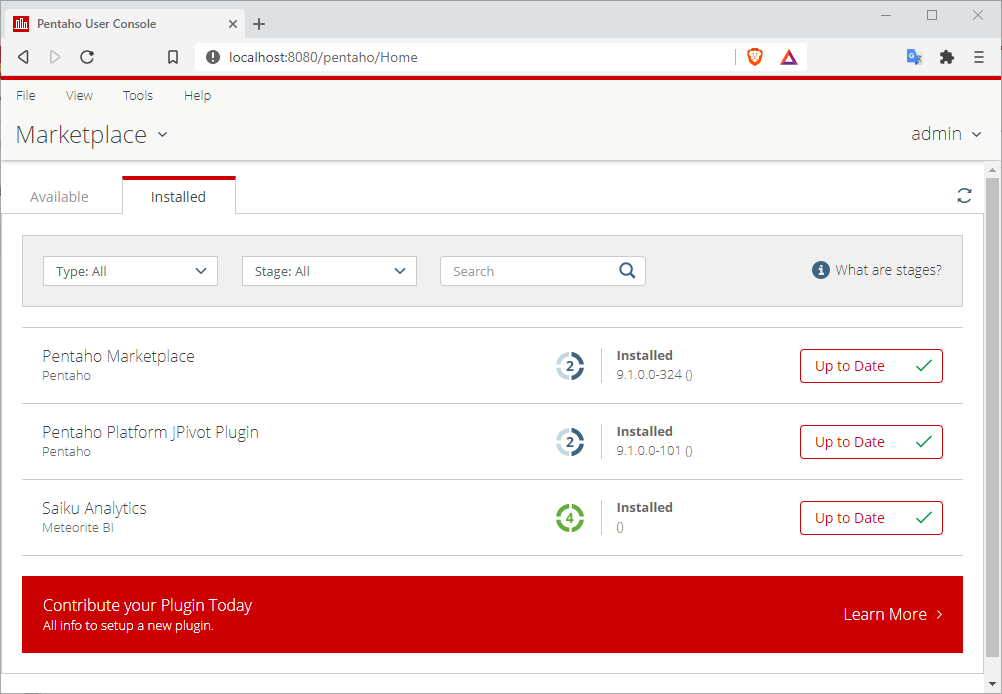
\includegraphics[scale=0.6]{Imagens/figura - pluginsaiku.png}
	\end{center}
	\legend{Fonte: Autor.}
\end{figure}

O ambiente para montagem dos relatórios pode ser conferido na \autoref{fig_saikuanalytics}.
Ele também utiliza o motor Mondrian para as consultas aos cubos ROLAP. Também permite que o usuário final elabore as próprias consultas com vários gráficos disponíveis e função \textit{drag in drop} tornando a experiência mais intuitiva, dispensando conhecimento prévio em SQL ou MDX. 

\newpage
\begin{figure}[htb]
	\caption{\label{fig_saikuanalytics}Ambiente de Relatórios do Saiku Analytics.}
	\begin{center}
	    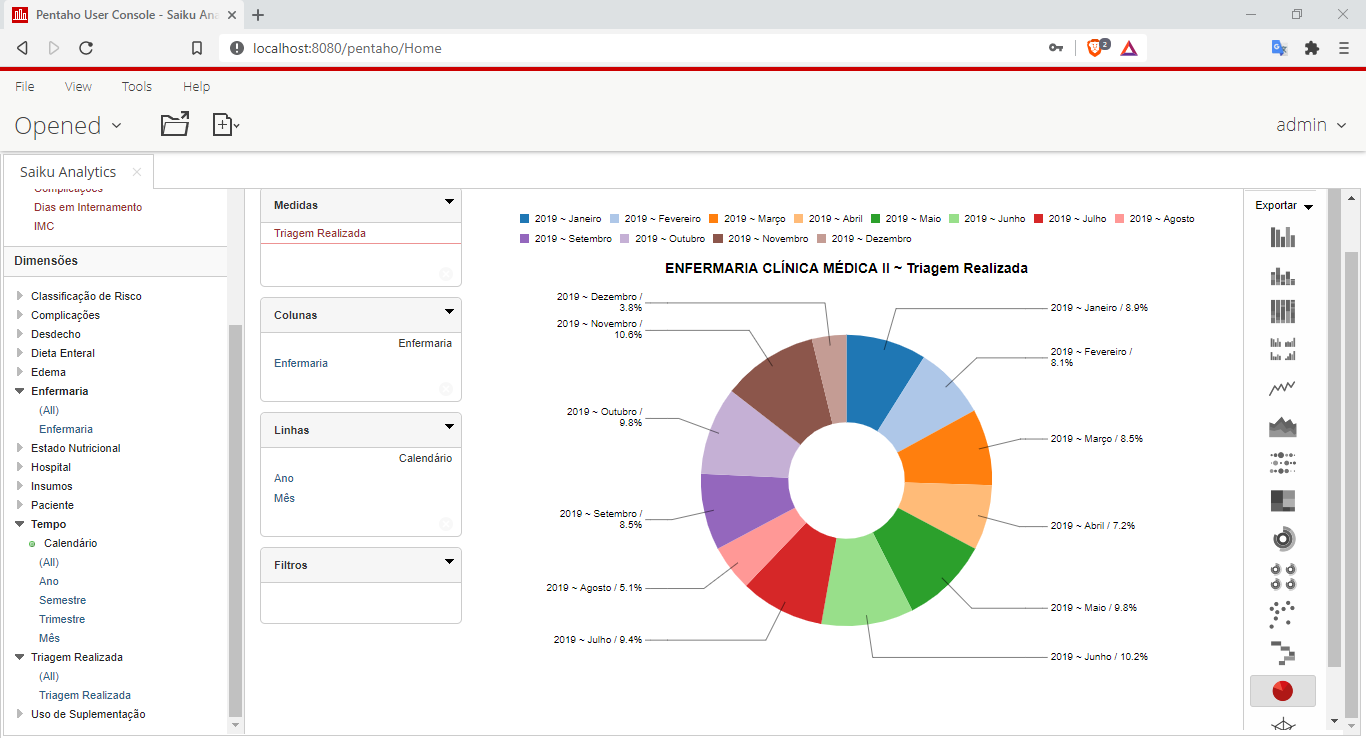
\includegraphics[scale=0.45]{Imagens/figura - saikudashboard.png}
	\end{center}
	\legend{Fonte: Autor.}
\end{figure}

\section{Resultados}

A plataforma de integração e análise de dados da Pentaho permite que as organizações acessem, preparem e analisem todos os dados de qualquer fonte, em qualquer ambiente \cite{pentahosite}. E o Saiku Analytics permite realizar análises complexas e poderosas usando uma interface fácil, arrastando e soltando as medidas e dimensões por meio do navegador criando relatórios detalhados e ótimas visualizações gráficas \cite{meteoribisite} A seguir estão  os resultados obtidos conforme as demandas solicitadas pela Unidade de Nutrição Clínica do HU-UFS.

\subsection{Relatórios e Dashboards Obtidos}
Com o ambiente de relatórios pronto e as consultas carregadas utilizando o Saiku Analytics foi possível gerar os relatórios com as informações solicitadas pela Unidade de Nutrição Clínica do Hospital Universitário. A \autoref{dashboard_TotalTriagensRealizadasHospitalAnoTabela}, mostra a quantidade de triagens nutricionais realizadas ao ano.

\begin{figure}[htb]
	\caption{\label{dashboard_TotalTriagensRealizadasHospitalAnoTabela}Quantidade de Triagens Nutricionais Realizadas ao Ano.}
	\begin{center}
	    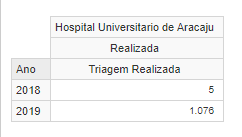
\includegraphics[scale=1]{Imagens/1.1.TotalTriagensRealizadasHospitalAnoTabela.png}
	\end{center}
	\legend{Fonte: Autor.}
\end{figure}
\newpage
A \autoref{dashboard_TotalTriagensRealizadasHospitalMesTabela}, mostra o relatório com a quantidade de triagens nutricionais realizadas por mês. 

\begin{figure}[htb]
	\caption{\label{dashboard_TotalTriagensRealizadasHospitalMesTabela}Quantidade de Triagens Nutricionais Realizadas ao Mês.}
	\begin{center}
	    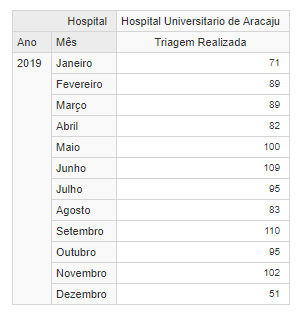
\includegraphics[scale=1]{Imagens/1.2.TotalTriagensRealizadasHospitalMesTabela.png}
	\end{center}
	\legend{Fonte: Autor.}
\end{figure}

\clearpage
A \autoref{dashboard_TotalTriagensRealizadasEnfermariaAnoBarras}, mostra o gráfico de barras sobre a quantidade de triagens nutricionais realizadas por enfermaria ao ano.

\begin{figure}[htb]
	\caption{\label{dashboard_TotalTriagensRealizadasEnfermariaAnoBarras}Quantidade de Triagens Nutricionais Realizadas Por Enfermaria ao Ano.}
	\begin{center}
	    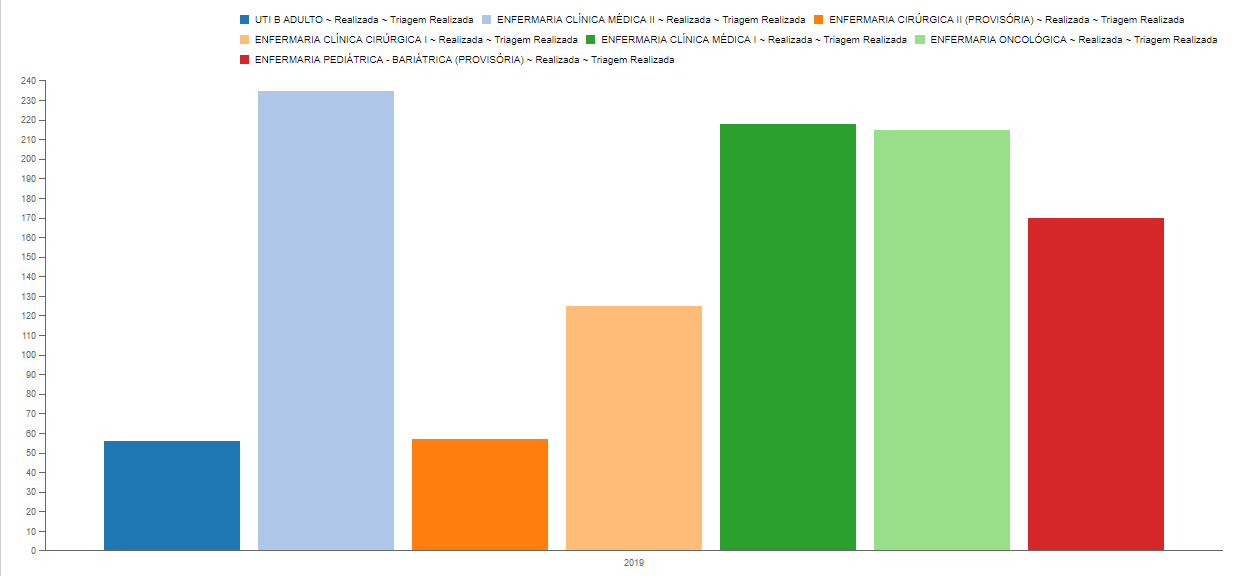
\includegraphics[scale=0.4]{Imagens/1.3.TotalTriagensRealizadasEnfermariaAnoBarras.png}
	\end{center}
	\legend{Fonte: Autor.}
\end{figure}

A \autoref{dashboard_TotalTriagensRealizadasEnfermariaMesLinhas}, contém um gráfico de linhas demonstrando a tendência de triagens nutricionais realizadas por enfermaria.

\begin{figure}[htb]
	\caption{\label{dashboard_TotalTriagensRealizadasEnfermariaMesLinhas}Tendência de Triagens Nutricionais Realizadas Por Enfermaria.}
	\begin{center}
	    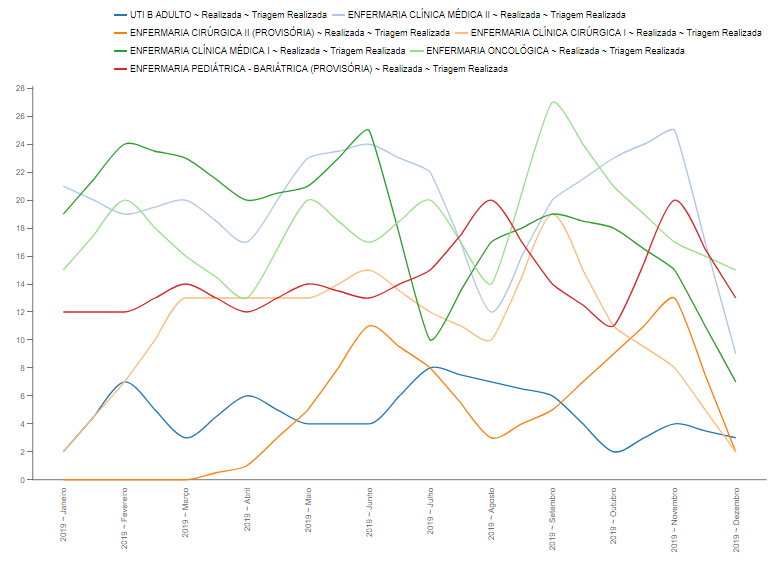
\includegraphics[scale=0.475]{Imagens/1.4.TotalTriagensRealizadasEnfermariaMesLinhas.png}
	\end{center}
	\legend{Fonte: Autor.}
\end{figure}
\clearpage
A \autoref{dashboard_PercentualClassificacaoRiscoHospitalAnoPizza}, mostra gráfico de pizza do percentual de pacientes segundo classificação de risco ao ano.

\begin{figure}[htb]
	\caption{\label{dashboard_PercentualClassificacaoRiscoHospitalAnoPizza}Percentual de Pacientes segundo Classificação de Risco ao Ano.}
	\begin{center}
	    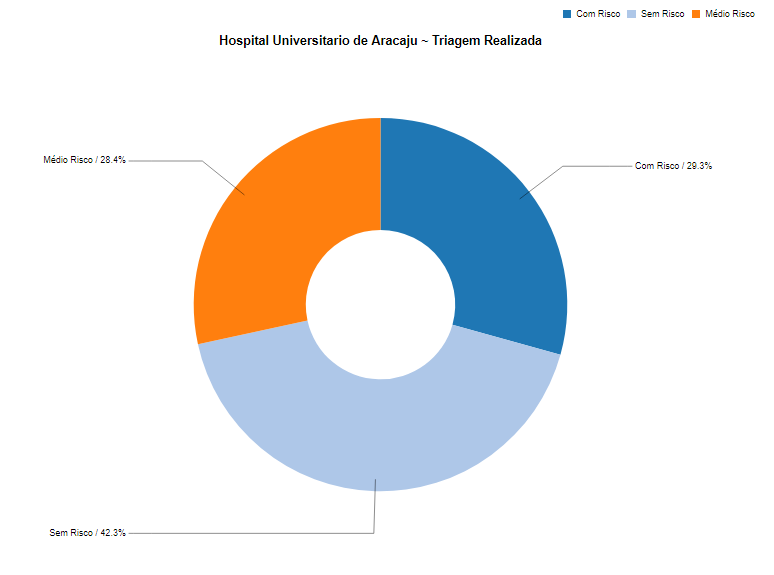
\includegraphics[scale=0.6]{Imagens/2.1.PercentualPacientesClassificacaoRiscoHospitalAnoPizza.png}
	\end{center}
	\legend{Fonte: Autor.}
\end{figure}

\clearpage
A \autoref{dashboard_PercentualPacientesClassificacaoRiscoHospitalMesPizza} mostra o percentual de classificação por triagem nutricional por mês.

\begin{figure}[htb]
	\caption{\label{dashboard_PercentualPacientesClassificacaoRiscoHospitalMesPizza}Percentual de Pacientes segundo Classificação de Risco detalhado por mês.}
	\begin{center}
	    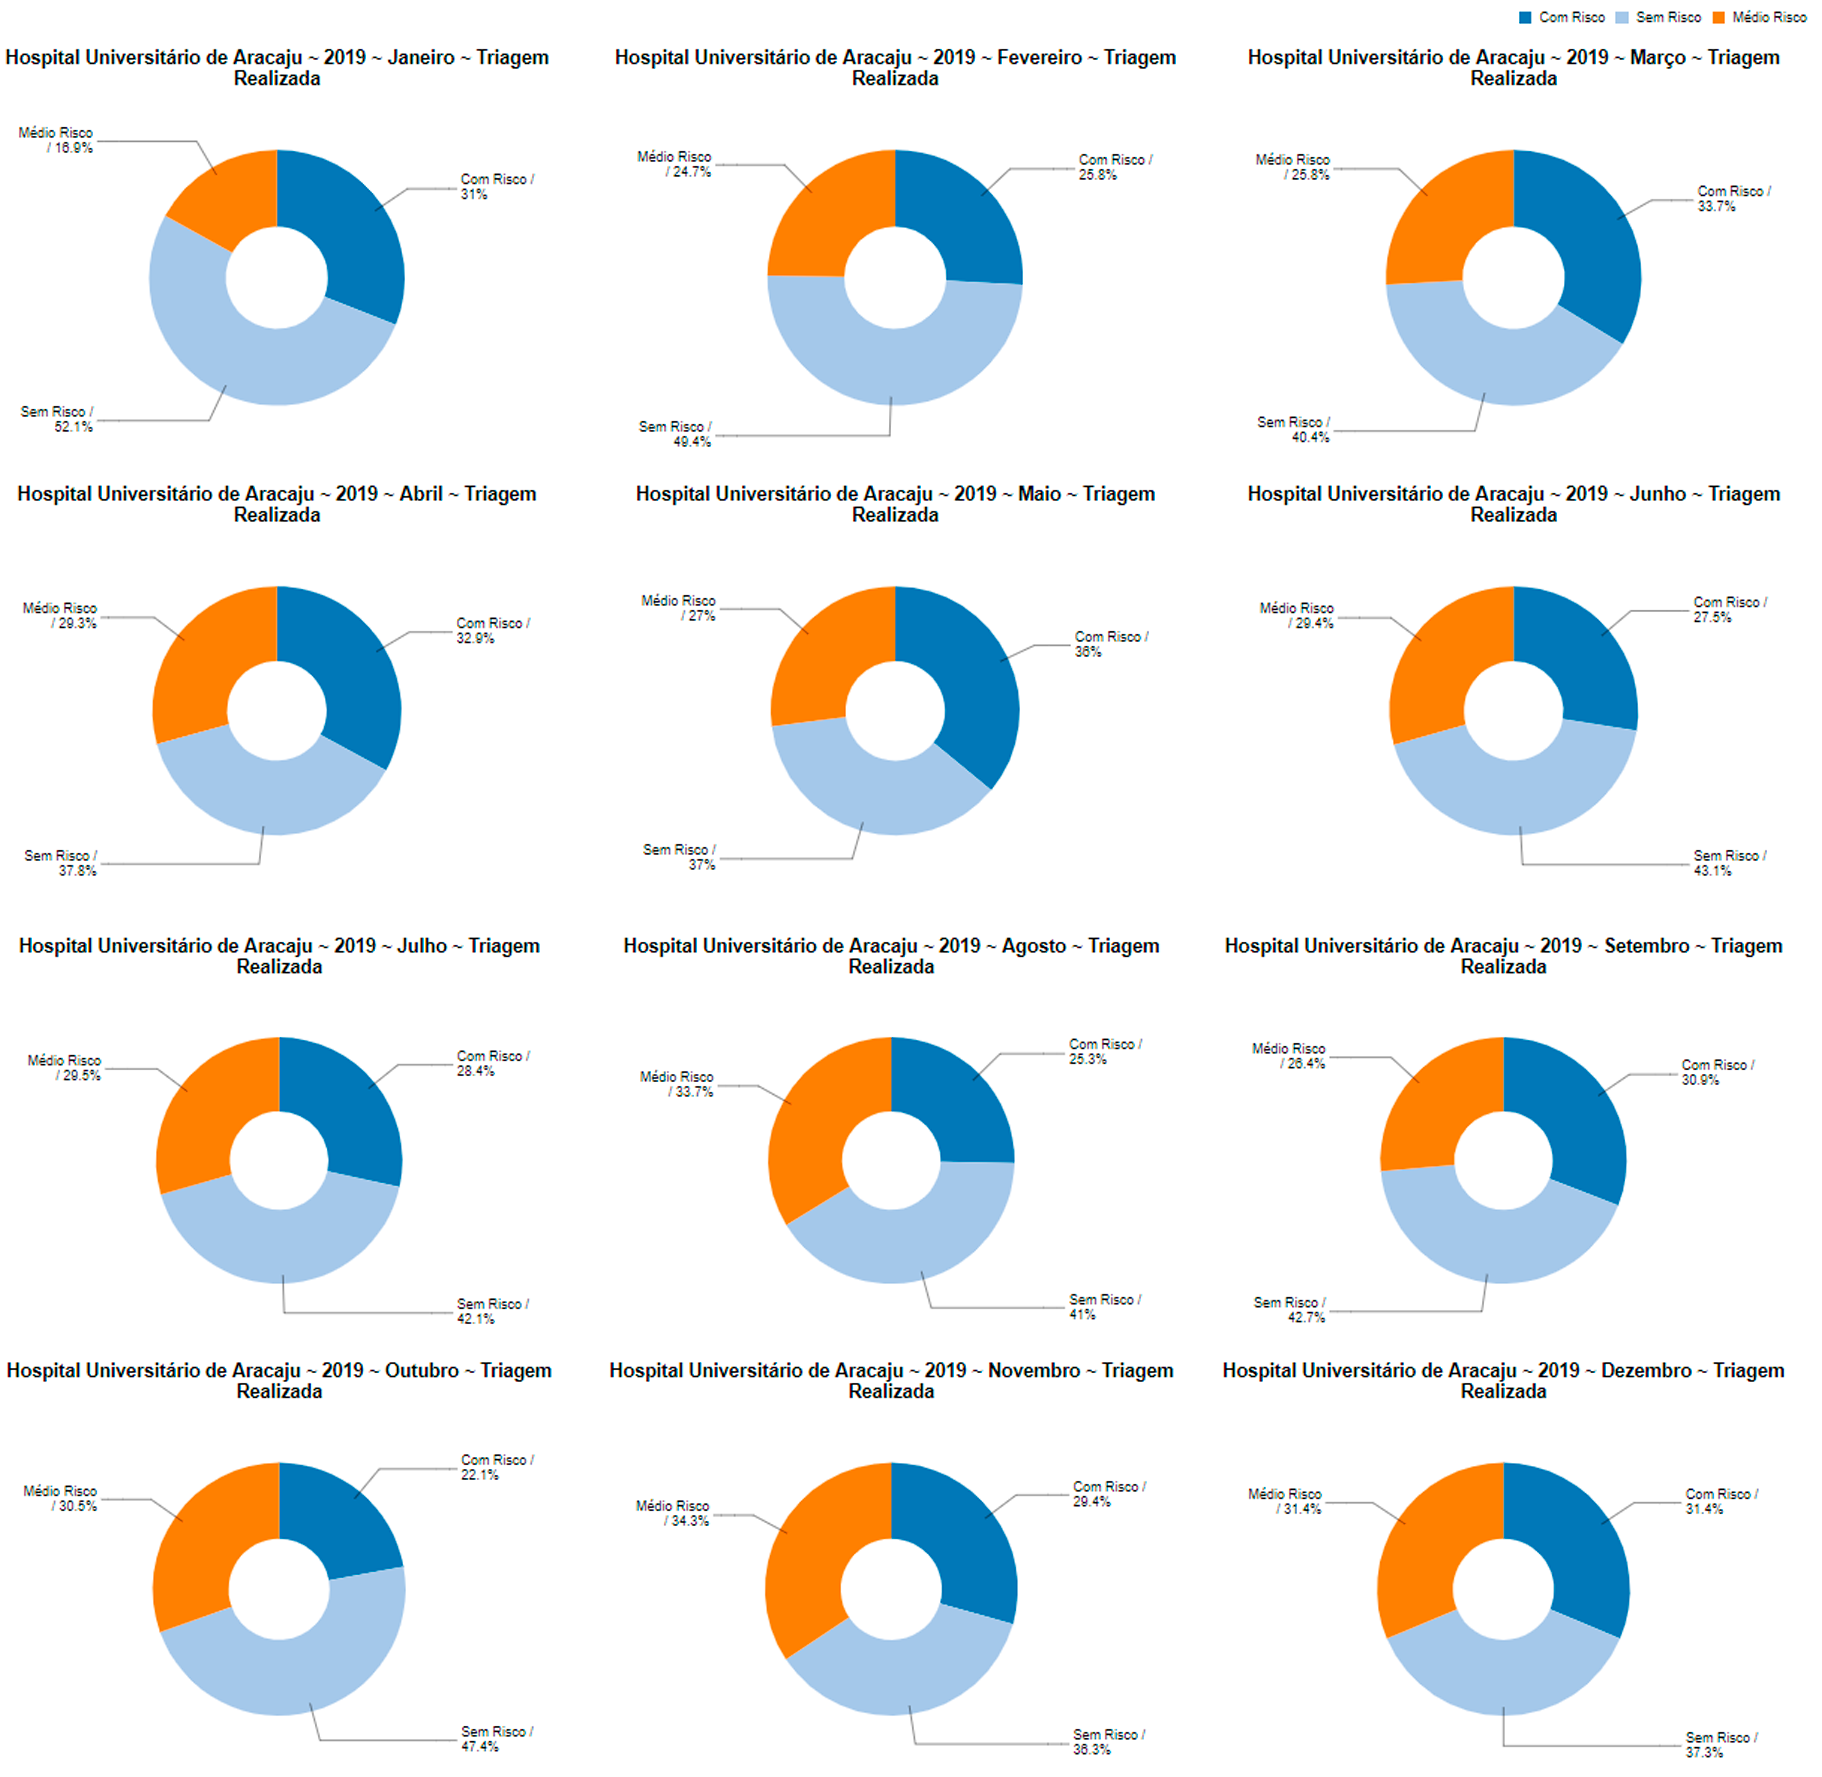
\includegraphics[scale=0.6]{Imagens/2.2.PercentualPacientesClassificacaoRiscoHospitalMesPizza.png}
	\end{center}
	\legend{Fonte: Autor.}
\end{figure}

\clearpage
A \autoref{dashboard_PercentualPacientesClassificacaoRiscoEnfermariaAnoPizza} mostra o percentual de classificação por triagem nutricional por mês.

\begin{figure}[htb]
	\caption{\label{dashboard_PercentualPacientesClassificacaoRiscoEnfermariaAnoPizza}Percentual de Pacientes segundo Classificação de Risco por Enfermaria ao Ano.}
	\begin{center}
	    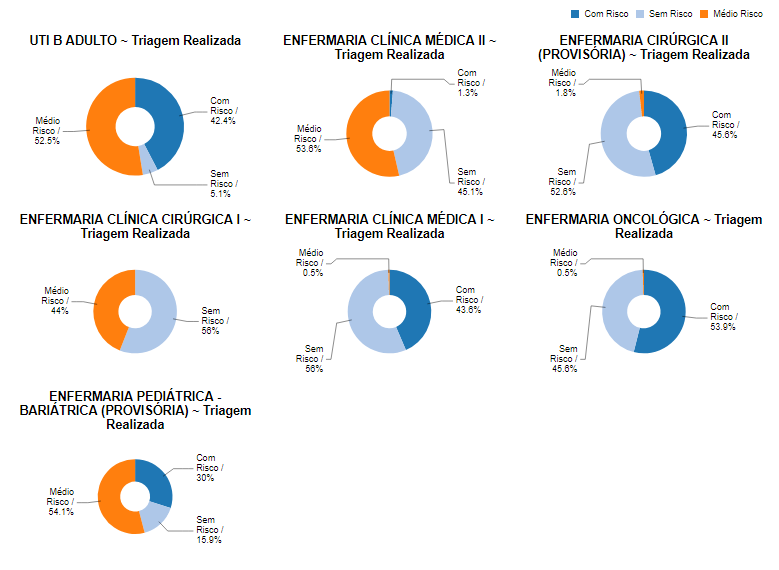
\includegraphics[scale=0.6]{Imagens/2.3.PercentualPacientesClassificacaoRiscoEnfermariaAnoPizza.png}
	\end{center}
	\legend{Fonte: Autor.}
\end{figure}

\clearpage
A \autoref{dashboard_PercentualPacientesClassificacaoRiscoEnfermariaMesLinha} mostra a tendência de pacientes segundo classificação por enfermaria por mês.

\begin{figure}[htb]
	\caption{\label{dashboard_PercentualPacientesClassificacaoRiscoEnfermariaMesLinha}Tendência de Pacientes segundo Classificação de Risco por Enfermaria detalhado por mês.}
	\begin{center}
	    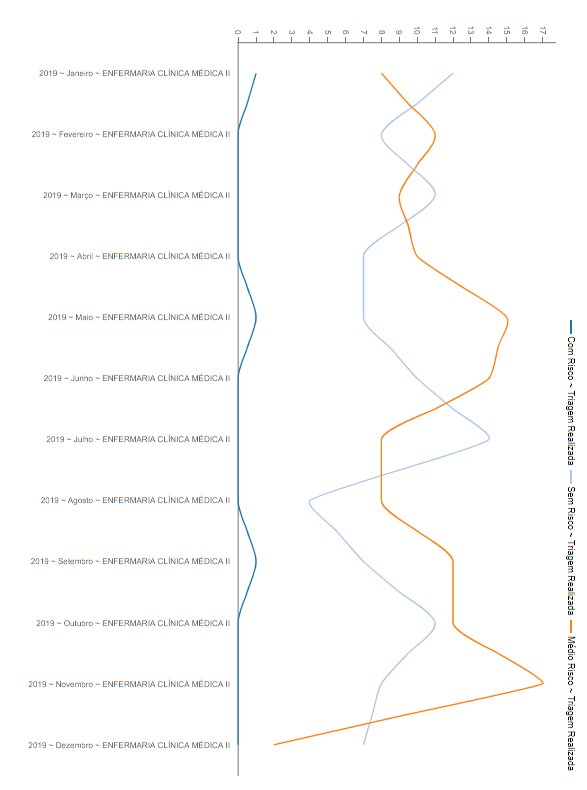
\includegraphics[scale=0.9]{Imagens/2.4.PercentualPacientesClassificacaoRiscoEnfermariaMesLinha.png}
	\end{center}
	\legend{Fonte: Autor.}
\end{figure}

\newpage
A \autoref{dashboard_PercentualPacienteEstadoNutricionalHospitalAnoPizza} mostra o percentual de pacientes segundo estado nutricional ao ano.

\begin{figure}[htb]
	\caption{\label{dashboard_PercentualPacienteEstadoNutricionalHospitalAnoPizza}Percentual de Pacientes segundo Estado Nutricional ao Ano.}
	\begin{center}
	    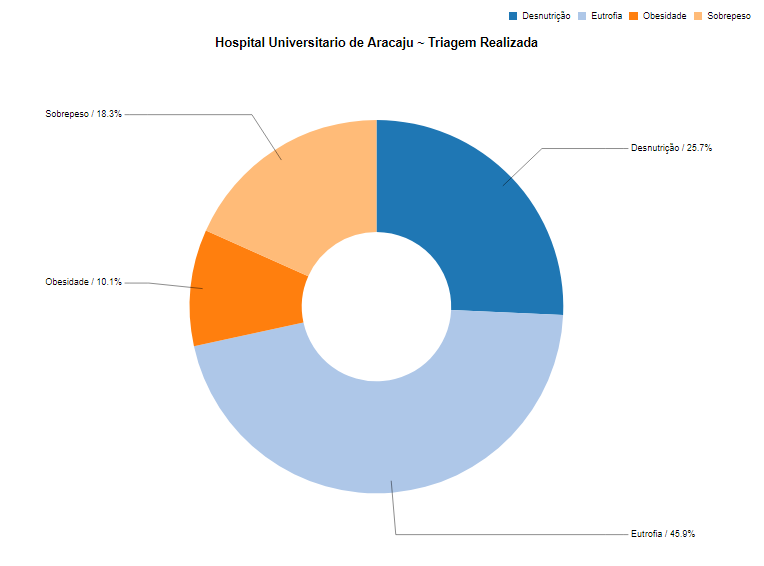
\includegraphics[scale=0.6]{Imagens/3.1.PercentualPacienteEstadoNutricionalHospitalAnoPizza.png}
	\end{center}
	\legend{Fonte: Autor.}
\end{figure}

\newpage
A \autoref{dashboard_PercentualPacienteEstadoNutricionalHospitalMesLinha} mostra o percentual de pacientes segundo estado nutricional por mês.

\begin{figure}[htb]
	\caption{\label{dashboard_PercentualPacienteEstadoNutricionalHospitalMesLinha}Percentual de Pacientes segundo Estado Nutricional detalhado por mês.}
	\begin{center}
	    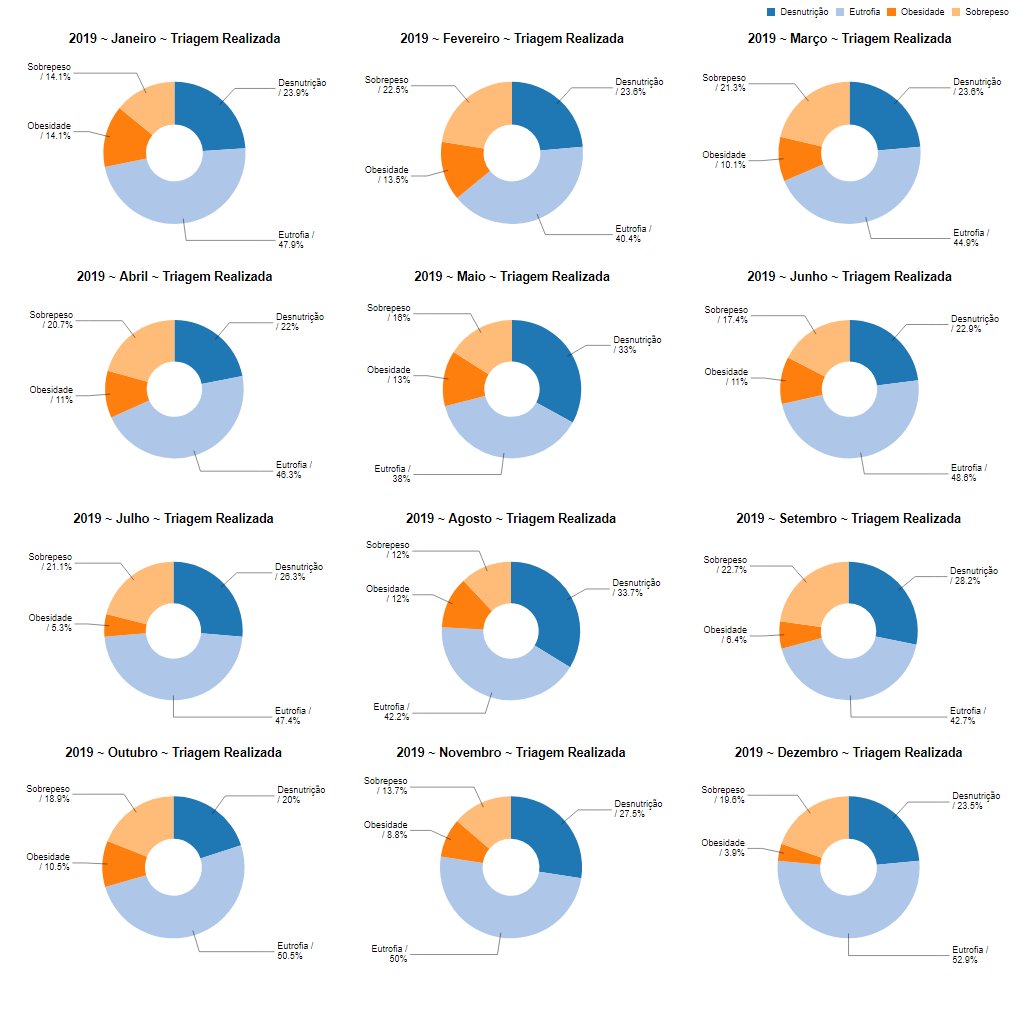
\includegraphics[scale=0.6]{Imagens/3.2.PercentualPacienteEstadoNutricionalHospitalMesLinha.png}
	\end{center}
	\legend{Fonte: Autor.}
\end{figure}

\newpage
A \autoref{dashboard_PercentualPacienteEstadoNutricionalEnfermariaAnoPizza} mostra o percentual de pacientes segundo estado nutricional por enfermaria ao ano.

\begin{figure}[htb]
	\caption{\label{dashboard_PercentualPacienteEstadoNutricionalEnfermariaAnoPizza}Percentual de Pacientes segundo Estado Nutricional por Enfermaria ao Ano.}
	\begin{center}
	    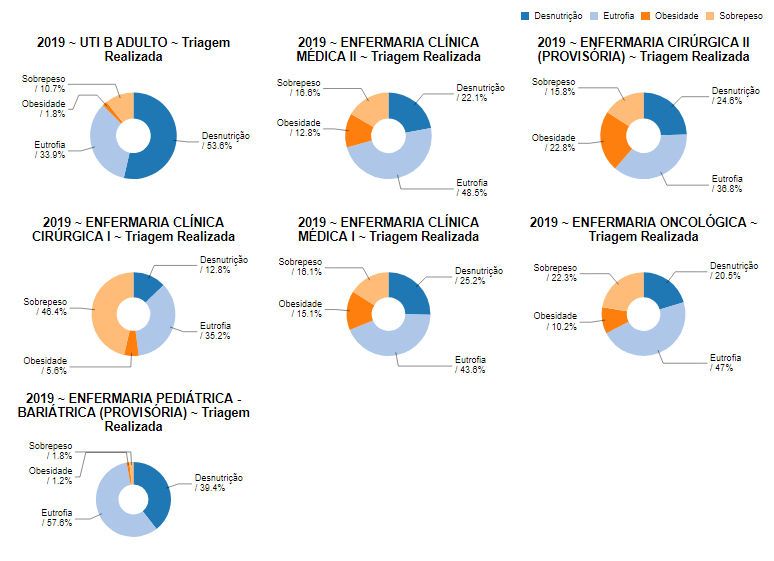
\includegraphics[scale=0.6]{Imagens/3.3.PercentualPacienteEstadoNutricionalEnfermariaAnoPizza.png}
	\end{center}
	\legend{Fonte: Autor.}
\end{figure}

\newpage
A \autoref{dashboard_PercentualPacienteEstadoNutricionalEnfermariaMesPizza} mostra a tendência de pacientes segundo estado nutricional por enfermaria por mês.

\begin{figure}[htb]
	\caption{\label{dashboard_PercentualPacienteEstadoNutricionalEnfermariaMesPizza}Tendência de Pacientes segundo Estado Nutricional por Enfermaria detalhado por mês.}
	\begin{center}
	    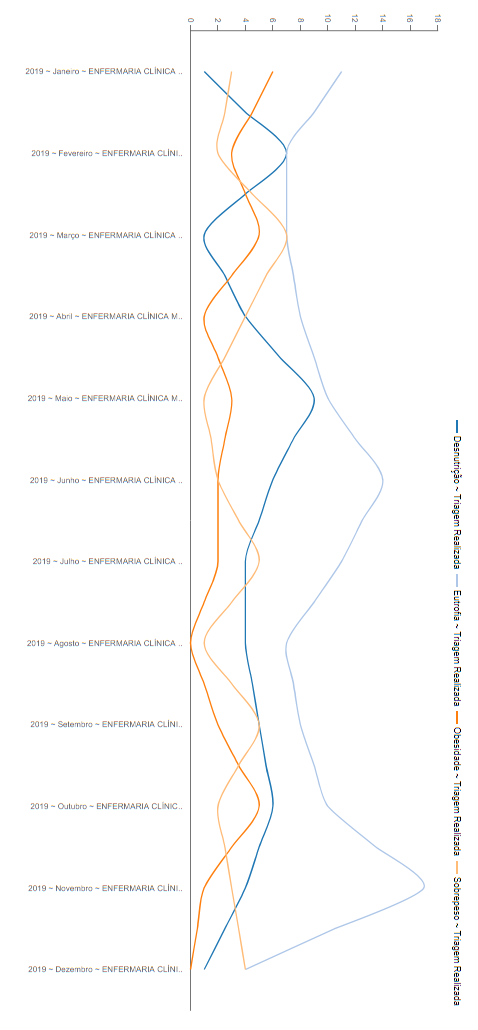
\includegraphics[scale=0.65]{Imagens/3.4.PercentualPacienteEstadoNutricionalEnfermariaMesPizza.png}
	\end{center}
	\legend{Fonte: Autor.}
\end{figure}

\newpage
A \autoref{dashboard_TotalUsoSuplementoHospitalAnoBarra} mostra a quantidade de pacientes em uso de suplementação ao ano.

\begin{figure}[htb]
	\caption{\label{dashboard_TotalUsoSuplementoHospitalAnoBarra}Quantidade de Pacientes em Uso de Suplemento.}
	\begin{center}
	    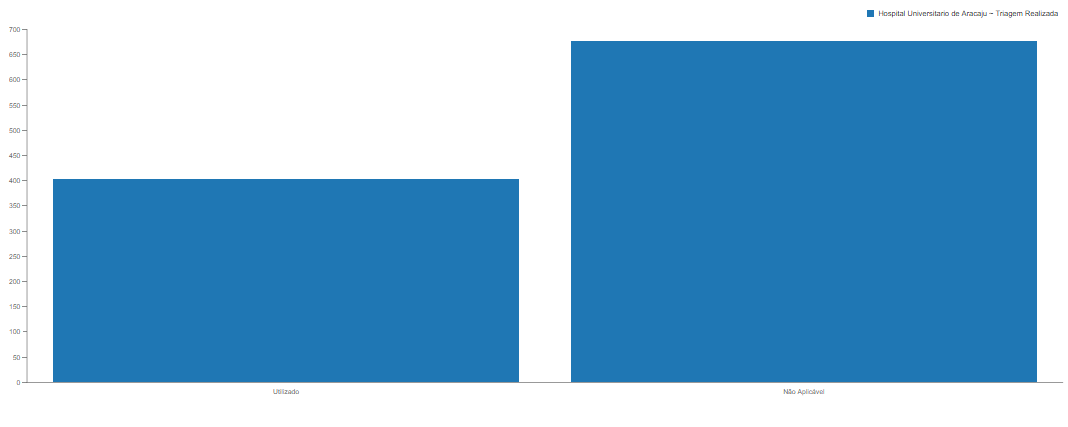
\includegraphics[scale=0.57]{Imagens/5.1.TotalUsoSuplementoHospitalAnoBarra.png}
	\end{center}
	\legend{Fonte: Autor.}
\end{figure}

A \autoref{dashboard_TotalUsoSuplementoEnfermariaAnoBarra} mostra a quantidade de pacientes em uso de suplementação por enfermaria.

\begin{figure}[htb]
	\caption{\label{dashboard_TotalUsoSuplementoEnfermariaAnoBarra}Quantidade de Pacientes em Uso de Suplemento por Enfermaria.}
	\begin{center}
	    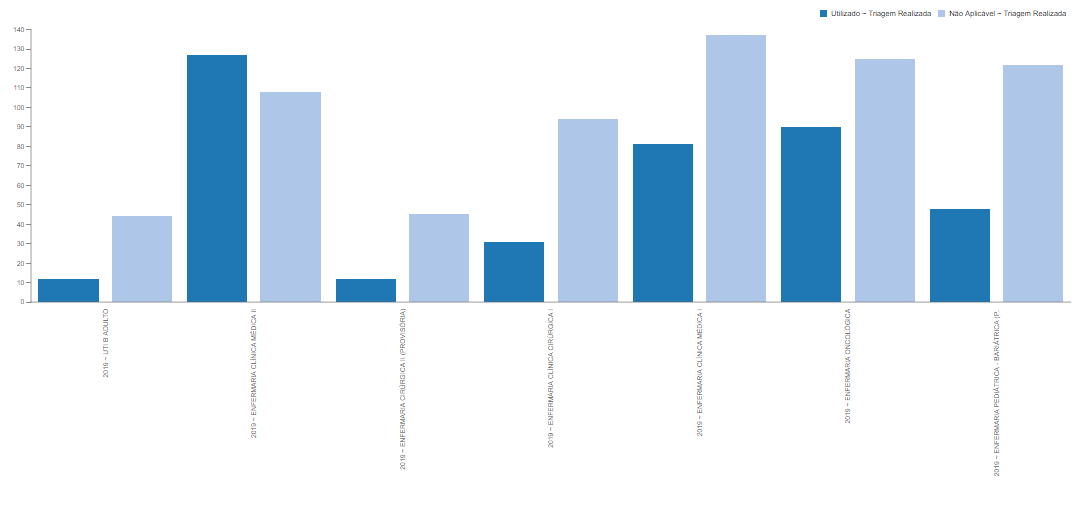
\includegraphics[scale=0.55]{Imagens/5.2.TotalUsoSuplementoEnfermariaAnoBarra.png}
	\end{center}
	\legend{Fonte: Autor.}
\end{figure}

\newpage
A \autoref{dashboard_PercentualPacienteUsoSuplementoHospitalAnoPizza} mostra o percentual de pacientes segundo uso de suplementação ao ano.

\begin{figure}[htb]
	\caption{\label{dashboard_PercentualPacienteUsoSuplementoHospitalAnoPizza}Percentual de Pacientes segundo Uso de Suplementação ao Ano.}
	\begin{center}
	    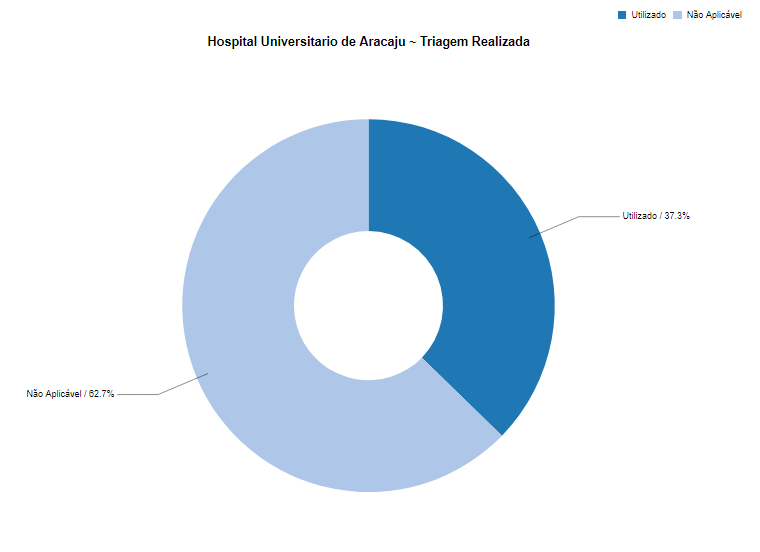
\includegraphics[scale=0.6]{Imagens/4.1.PercentualPacienteUsoSuplementoHospitalAnoPizza.png}
	\end{center}
	\legend{Fonte: Autor.}
\end{figure}

\newpage
A \autoref{dashboard_PercentualPacienteUsoSuplementoEnfermariaAnoPizza} mostra o percentual de pacientes segundo uso de suplementação por enfermaria ao ano.

\begin{figure}[htb]
	\caption{\label{dashboard_PercentualPacienteUsoSuplementoEnfermariaAnoPizza}Percentual de Pacientes segundo Uso de Suplementação por Enfermaria ao Ano.}
	\begin{center}
	    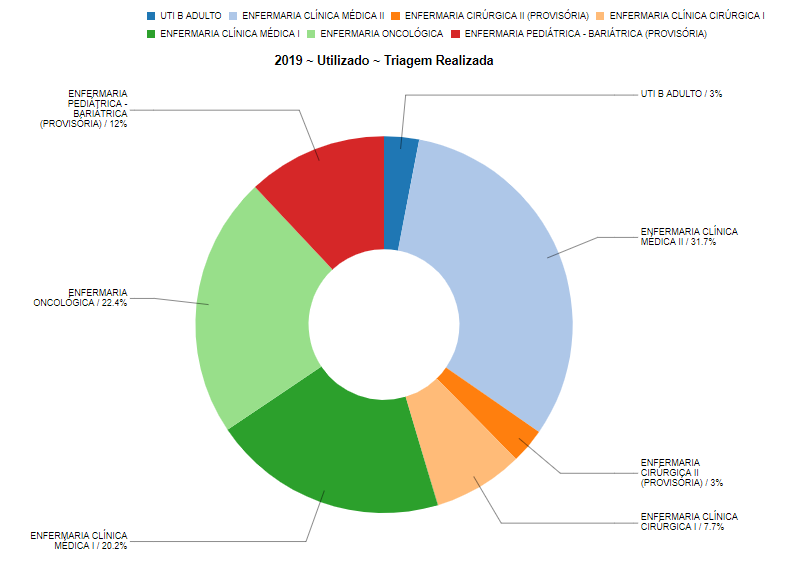
\includegraphics[scale=0.75]{Imagens/4.3.PercentualPacienteUsoSuplementoEnfermariaAnoPizza.png}
	\end{center}
	\legend{Fonte: Autor.}
\end{figure}

\newpage
A \autoref{dashboard_PercentualPacienteUsoSuplementoEnfermariaMesLinha} mostra a tendência de pacientes segundo uso de suplementação por enfermaria ao ano.

\begin{figure}[htb]
	\caption{\label{dashboard_PercentualPacienteUsoSuplementoEnfermariaMesLinha}Tendência de Pacientes segundo Uso de Suplementação por Enfermaria detalhado por mês.}
	\begin{center}
	    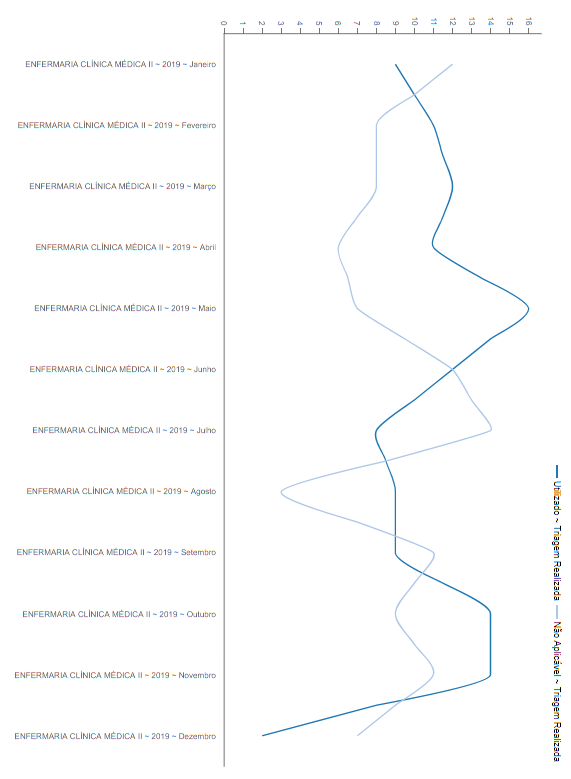
\includegraphics[scale=0.9]{Imagens/4.4.PercentualPacienteUsoSuplementoEnfermariaMesLinha.png}
	\end{center}
	\legend{Fonte: Autor.}
\end{figure}

\newpage
A \autoref{dashboard_TotalUsoSuplementoMediaDeDiasInternadoHospitalMesBarra} mostra um comparativo entre os pacientes que utilizam suplementação com a média de dias em internamento.

\begin{figure}[htb]
	\caption{\label{dashboard_TotalUsoSuplementoMediaDeDiasInternadoHospitalMesBarra}Comparativo de pacientes que utilizam Suplementação com média de dias internado.}
	\begin{center}
	    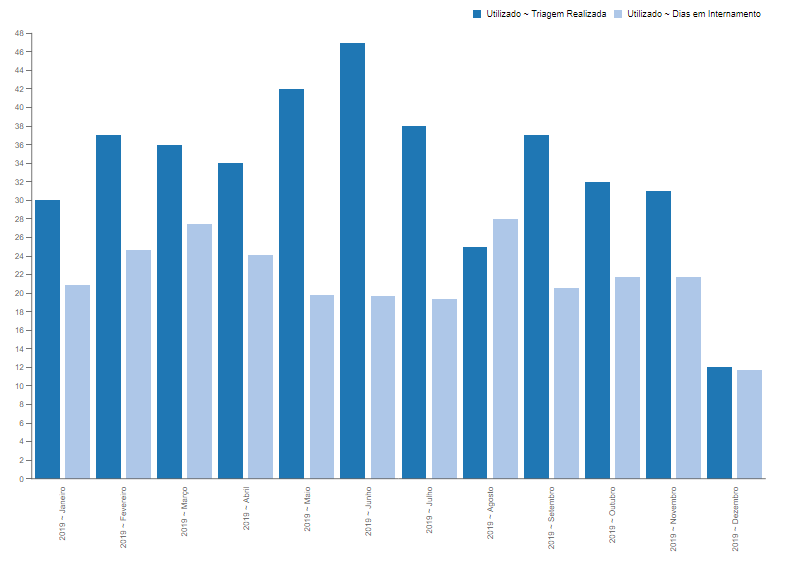
\includegraphics[scale=0.35]{Imagens/6.1.TotalUsoSuplementoMediaDeDiasInternadoHospitalMesBarra.png}
	\end{center}
	\legend{Fonte: Autor.}
\end{figure}

%\newpage
A \autoref{dashboard_TotalUsoSuplementoMediaDeDiasInternadoEnfermariaMesBarra} mostra um comparativo entre os pacientes que utilizam suplementação com a média de dias em internamento por enfermaria.

\begin{figure}[htb]
	\caption{\label{dashboard_TotalUsoSuplementoMediaDeDiasInternadoEnfermariaMesBarra}Comparativo de pacientes que utilizam Suplementação com média de dias internado por
enfermaria.}
	\begin{center}
	    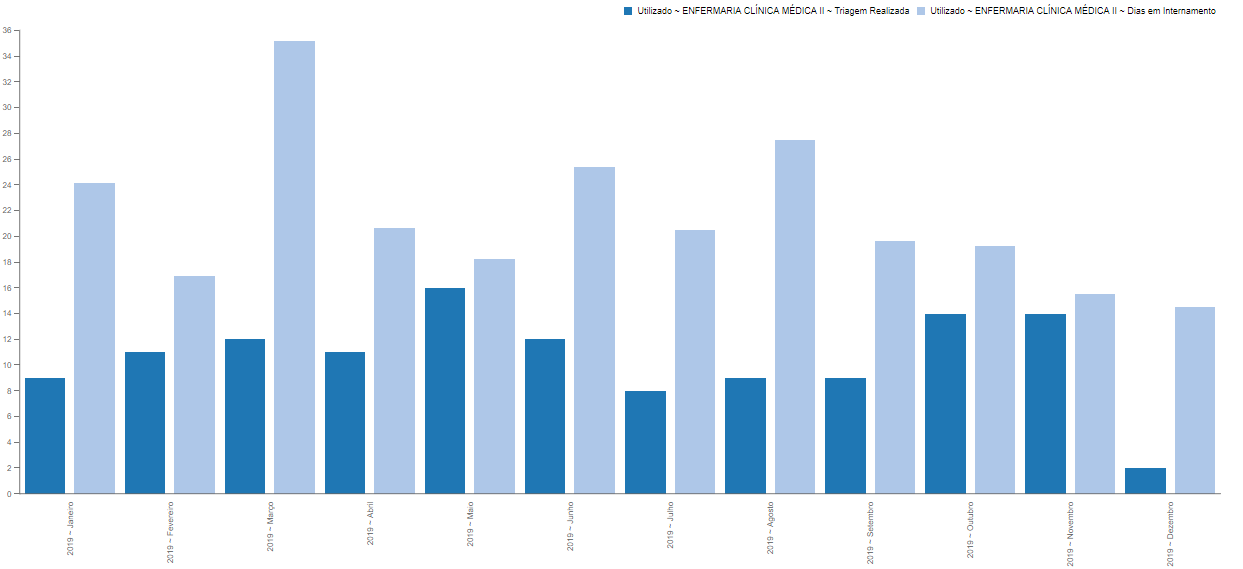
\includegraphics[scale=0.35]{Imagens/6.2.TotalUsoSuplementoMediaDeDiasInternadoEnfermariaMesBarra.png}
	\end{center}
	\legend{Fonte: Autor.}
\end{figure}

\section{Considerações do capítulo}
Neste capítulo foi apresentado o processo de construção do ambiente BI para a unidade de nutrição do HU. Foram detalhados aspectos técnicos e escopo do projeto. Foi descrito o processo de ETL para monitoramento dos indicadores solicitados pela unidade de nutrição do hospital, a modelagem de um cubo lógico e o desenvolvimento de \textit{querys} de consulta que são utilizadas na plataforma Pentaho, bem como a construção dos \textit{dashboards} para interpretação dos dados coletados pelo departamento. O próximo capítulo apresenta as considerações finais deste trabalho.

% ---
\chapter{Considerações Finais}
% ---
Este trabalho apresentou o desenvolvimento de um ambiente de \textit{Business Intelligence} para a Unidade de Nutrição Clínica do Hospital Universitário de Aracaju, transformando os dados gerados pela unidade em informação para apoiar a gestão do departamento na tomada de decisão gerencial.

O estado nutricional do paciente internado impacta diretamente na melhora ou piora da sua condição clínica. E mensurar, avaliar e melhorar os indicadores de qualidade do processo de terapia nutricional é imprescindível para melhorar o atendimento aos usuários do serviço de saúde hospitalar. O que consequentemente também melhora a qualidade de vida do paciente, ajudando a reduzir seu tempo de internação, reduzindo gastos hospitalares e possibilitando que os recursos sejam melhor aplicados. O ambiente de BI desenvolvido impacta o processo de análise da gestão HU provendo \textit{dashboards} com indicadores calculados em diferentes dimensões ampliando o campo de alcance das informações.

O desenvolvimento ambiente BI foi apoiado por algumas etapas. Uma revisão sistemática foi realizada para extração de informações relevantes de trabalhos publicados em bases acadêmicas que tratam da aplicação de sistemas de apoio a decisão para nutrição em ambiente hospitalar. Ocorreram reuniões e visitas a Unidade de Nutrição do HU com o objetivo de elencar requisitos para desenvolvimento dos \textit{dashboards}. 

Espera-se que a utilização do BI no monitoramento dos indicadores de terapia nutricional contribua para a instituição, sendo uma fonte de informações confiáveis e eficazes para a tomada de decisão. O sistema BI proporciona análise analítica de informações para auxiliar a gestão hospitalar numa melhor condução da prestação dos serviços hospitalares.

Para trabalhos futuros, sugere-se avaliar o impacto do ambiente BI no cumprimento de demandas de decisão da gestão da unidade, conectar o Sistema de Informação Nutricional que está sendo implantado na unidade, em substituição ao atual modelo de registro de informações em planilhas eletrônicas, incluindo assim uma fonte de dados integra e atualizada do departamento, afim de responder com informações importantes no menor tempo possível. Possibilitando a criação de tarefas de ETL agendadas para carga de informações no Data Warehouse.
%\chapter{Customização DCOMP}

\section{Lista de códigos}

Usado para criar a lista de códigos, adicionar sintaxe highlight, enumerar as linhas e colorir o fundo, para dar destaque a implementação.

Sintaxe básica:
\begin{verbatim}
\begin{codigo}[!htb]
    \caption{Espaço para o título do código}
    \label{Espaço para o label do código, para ser usado na referência}  
    \begin{lstlisting}[language = Linguagem de programação a ser usada]
        <CÓDIGO>
    \end{lstlisting}
\end{codigo}
\end{verbatim}

\begin{codigo}[htb]
  \caption{Código PHP}
  \label{codigophp}
  \begin{lstlisting}[language = php]
       <?php

       echo '%*Olá mundo*)!';
       print '%*Olá mundo*)!';
  \end{lstlisting}
\end{codigo}

\begin{codigo}
  \caption{Código python}
  \label{codigopython}
  \begin{lstlisting}[language = python]
    import numpy as np
 
    def incmatrix(genl1, genl2):
        m = len(genl1)
        n = len(genl2)
        M = None #to become the incidence matrix
        VT = np.zeros((n*m,1), int)  #dummy variable
 
        #compute the bitwise xor matrix
        M1 = bitxormatrix(genl1)
        M2 = np.triu(bitxormatrix(genl2),1) 
 
        for i in range(m-1):
            for j in range(i+1, m):
                [r,c] = np.where(M2 == M1[i,j])
                for k in range(len(r)):
                    VT[(i)*n + r[k]] = 1;
                    VT[(i)*n + c[k]] = 1; 
                    VT[(j)*n + r[k]] = 1;
                    VT[(j)*n + c[k]] = 1;
 
                    if M is None:
                        M = np.copy(VT)
                    else:
                        M = np.concatenate((M, VT), 1)
 
                    VT = np.zeros((n*m,1), int)
 
        return M
\end{lstlisting}
\end{codigo}

\begin{codigo}
  \caption{Codigo Java}
  \begin{lstlisting}[language = Java]
    public class Factorial{
        public static void main(String[] args){   
            final int NUM_FACTS = 100;
            for(int i = 0; i < NUM_FACTS; i++)
                System.out.println( i + "! is " + factorial(i) + factorial(i) factorial(i) factorial(i));
        }

        public static int factorial(int n){
            int result = 1;
            for(int i = 2; i <= n; i++)
                result *= i;
            return result;
        }
    }
\end{lstlisting}
\end{codigo}



\section{Lista de Algoritmos}

Usado para criar a lista de algoritmos ou pseudocodigos.

Sintaxe básica:
\begin{verbatim}
\begin{algoritmo}[!htb]
    \caption{Espaço para o título do algoritmo ou pseudocodigo}
    \label{label do do algoritmo ou pseudocodigo, para ser usado na referência}  
    <ESPAÇO RESERVADO PARA USAR SEU PACOTE FAVORITO DE CÓDIGOS>
\end{algoritmo}
\end{verbatim}


\begin{algoritmo}[htb]
	\caption{Algoritmo exemplo}
	\label{alg1}
	\begin{algorithm}[H]
 	\KwData{this text}
 	\KwResult{how to write algorithm with \LaTeX2e }
 	initialization\;
 	\While{not at end of this document}{
  		read current\;
  		\eIf{understand}{
   			go to next section\;
   			current section becomes this one\;
   		}{
   			go back to the beginning of current section\;
  		}
 	}
	\end{algorithm}
\end{algoritmo}

%\chapter{Conclusão}

\lipsum[31-33]

\phantompart
\bibliography{Bibliografia}

%%%%%%%%%%%%%%%%%%%%%%%%%%%%%%%%%%%%%%%%%%%%%%%%%%%%%%%%%%%%%%%%%%%%%%%%%%
% ELEMENTOS PÓS-TEXTUAIS
%%%%%%%%%%%%%%%%%%%%%%%%%%%%%%%%%%%%%%%%%%%%%%%%%%%%%%%%%%%%%%%%%%%%%%%%%%

\postextual

\renewcommand{\chapnumfont}{\chaptitlefont}
\renewcommand{\afterchapternum}{}
\begin{apendicesenv}

% Imprime uma página indicando o início dos apêndices
% \partapendices



\end{apendicesenv}

\begin{anexosenv}


% Imprime uma página indicando o início dos anexos
% \partanexos




\end{anexosenv}


\end{document}